\PassOptionsToPackage{unicode=true}{hyperref} % options for packages loaded elsewhere
\PassOptionsToPackage{hyphens}{url}
%
\documentclass[12pt,italian,]{report}
\usepackage{lmodern}
\usepackage{amssymb,amsmath}
\usepackage{ifxetex,ifluatex}
\usepackage{fixltx2e} % provides \textsubscript
\ifnum 0\ifxetex 1\fi\ifluatex 1\fi=0 % if pdftex
  \usepackage[T1]{fontenc}
  \usepackage[utf8]{inputenc}
  \usepackage{textcomp} % provides euro and other symbols
\else % if luatex or xelatex
  \usepackage{unicode-math}
  \defaultfontfeatures{Ligatures=TeX,Scale=MatchLowercase}
\fi
% use upquote if available, for straight quotes in verbatim environments
\IfFileExists{upquote.sty}{\usepackage{upquote}}{}
% use microtype if available
\IfFileExists{microtype.sty}{%
\usepackage[]{microtype}
\UseMicrotypeSet[protrusion]{basicmath} % disable protrusion for tt fonts
}{}
\IfFileExists{parskip.sty}{%
\usepackage{parskip}
}{% else
\setlength{\parindent}{0pt}
\setlength{\parskip}{6pt plus 2pt minus 1pt}
}
\usepackage{hyperref}
\hypersetup{
            pdftitle={Progetto Usabilità e User Experience 2018/2019},
            pdfauthor={Filippo Bartolini; Adamo Fapohunda; Giacomo Leidi; Cristian Castiglione},
            pdfborder={0 0 0},
            breaklinks=true}
\urlstyle{same}  % don't use monospace font for urls
\usepackage{longtable,booktabs}
% Fix footnotes in tables (requires footnote package)
\IfFileExists{footnote.sty}{\usepackage{footnote}\makesavenoteenv{longtable}}{}
\usepackage{graphicx,grffile}
\makeatletter
\def\maxwidth{\ifdim\Gin@nat@width>\linewidth\linewidth\else\Gin@nat@width\fi}
\def\maxheight{\ifdim\Gin@nat@height>\textheight\textheight\else\Gin@nat@height\fi}
\makeatother
% Scale images if necessary, so that they will not overflow the page
% margins by default, and it is still possible to overwrite the defaults
% using explicit options in \includegraphics[width, height, ...]{}
\setkeys{Gin}{width=\maxwidth,height=\maxheight,keepaspectratio}
\setlength{\emergencystretch}{3em}  % prevent overfull lines
\providecommand{\tightlist}{%
  \setlength{\itemsep}{0pt}\setlength{\parskip}{0pt}}
\setcounter{secnumdepth}{0}
% Redefines (sub)paragraphs to behave more like sections
\ifx\paragraph\undefined\else
\let\oldparagraph\paragraph
\renewcommand{\paragraph}[1]{\oldparagraph{#1}\mbox{}}
\fi
\ifx\subparagraph\undefined\else
\let\oldsubparagraph\subparagraph
\renewcommand{\subparagraph}[1]{\oldsubparagraph{#1}\mbox{}}
\fi

% set default figure placement to htbp
\makeatletter
\def\fps@figure{htbp}
\makeatother

\ifnum 0\ifxetex 1\fi\ifluatex 1\fi=0 % if pdftex
  \usepackage[shorthands=off,main=italian]{babel}
\else
  \usepackage{polyglossia}
  \setmainlanguage[]{italian}
\fi

\title{Progetto Usabilità e User Experience 2018/2019}
\author{Filippo Bartolini \and Adamo Fapohunda \and Giacomo Leidi \and Cristian Castiglione}
\date{}

\begin{document}
\maketitle

{
\setcounter{tocdepth}{2}
\tableofcontents
}
\section{introduzione}\label{introduzione}
Kids Experience è un applicativo web legato al sito madre Kiabi.

Kiabi è un'azienda francese di e-commerce e distribuzione di
abbigliamento pronto moda, facente parte del gruppo Mulliez. Il suo
slogan \emph{``La moda a piccoli prezzi''} si basa su prodotti a prezzi
accessibili per tutta la famiglia.

Kids Experience offre ai clienti la possibilità di personalizzare
autonomamente megliette per bambini e ragazzi, da 3 a 12 anni, andando
ad ampliare la vasta gamma di prodotti offerti da Kiabi.

L'idea di base e il punto di forza di questa nuova categoria di prodotti
è l'estrema personalizzazione del capo d'abbigliamento scelto da parte
dell'utente.
\section{Ricerca etnografica}\label{ricerca-etnografica}
È possibile subito osservare come i bisogni che Kids Experience andrà a
soddisfare non si trovino nei primi livelli della gerarchia di Maslow,
ma si identifichino nel livello intermedio della gerarchia: il livello
di \emph{appartenenza}.

Successivamente si è fatta un'analisi del mercato dell'abbigliamento,
analizzando alcuni competitors attraverso dati reperiti online.
Precisamente, come si evince dalla Fig \ref{abbigliamo_generico}, per quanto riguarda il
mercato italiano il maggiore esponente è risultato essere Zara, mentre Kiabi si
posiziona al terzo posto.

\begin{figure}[h]
\centering
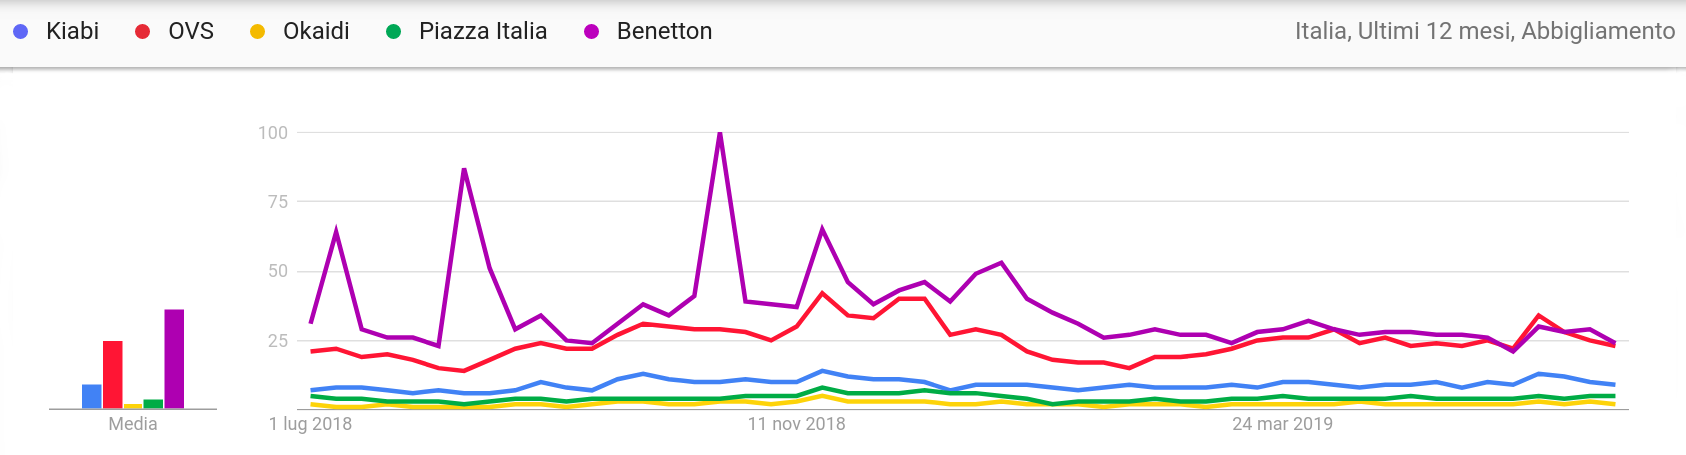
\includegraphics{img/abbigliamento_generico.png}
\caption{Ricerca di mercato - abbigliamento}
\label{abbigliamo_generico}
\end{figure}

Per quanto riguarda il mercato dell'abbigliamento da bambino, Kiabi perde un ulteriore posizione passando dal terzo al quarto posto, come mostrato in Fig. \ref{abbigliamento_bambino}.

\begin{figure}[h]
\centering
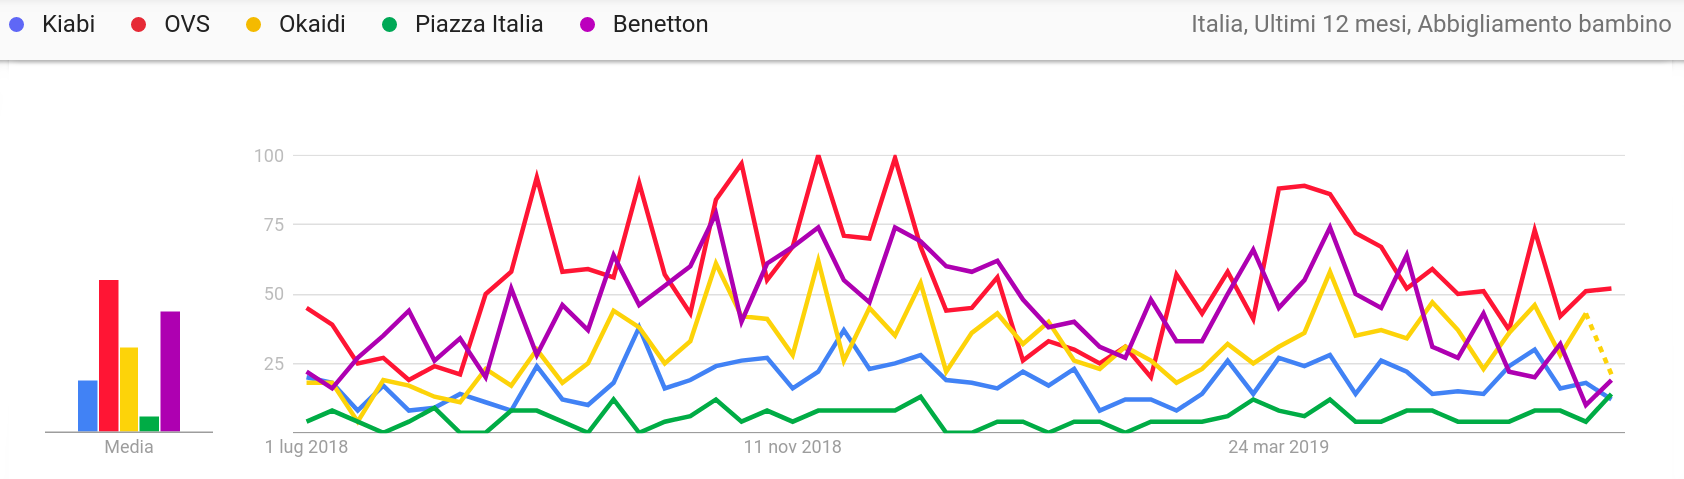
\includegraphics{img/abbigliamento_bambino.png}
\caption{Ricerca di mercato - abbigliamento bambino}
\label{abbigliamento_bambino}
\end{figure}

Dopo un'attenta analisi abbiamo deciso di prendere Kiabi come azienda
madre, con l'obiettivo di rilanciarla sul mercato dell'abbigliamento per
bambina/o tramite l'aggiunta di nuove features da noi ideate e proposte
al Project Manager Mulliez.

L'idea di progettare magliette estremamente perzonalizzabili solo per
bambini, nasce dalla semplicità del capo dettati dai minimi vincoli fisici
(i.e. taglia) del target. Questo permette di garantire all'utente
un'ampia gamma di personalizzazioni senza dover complicare eccessivamente
il processo di manifattura.
\section{Blueprint}\label{Blueprint}
Le blueprint sono semplici diagrammi che definiscono l'organizzazione dei contenuti e come le varie componenti interagiscono tra di loro.

Saranno presentate quattro blueprint che mostrano rispettivamente:

\begin{enumerate}
\def\labelenumi{\arabic{enumi}.}
\tightlist
\item
  Creazione di un nuovo modello
\item
  Organizzazione delle azioni disponibili per un utente loggato
\item
  Organizzazione delle azioni disponibili per un utente non loggato
\end{enumerate}
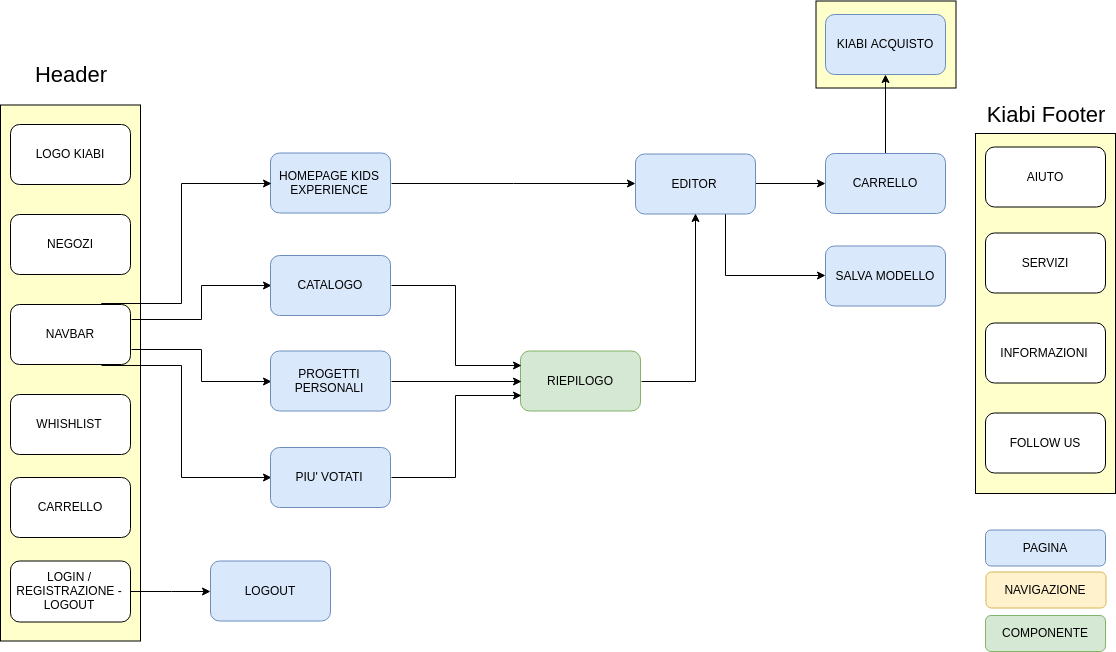
\includegraphics{blueprints/Utente_loggato.png}
\\
\\
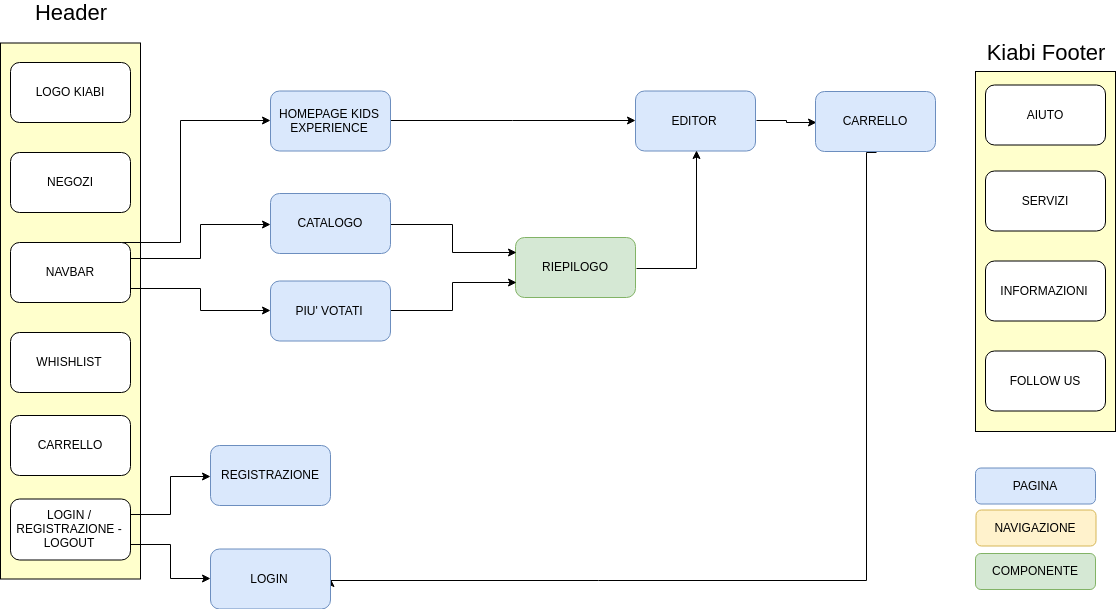
\includegraphics{blueprints/Utente_non_loggato.png}
\\
\\
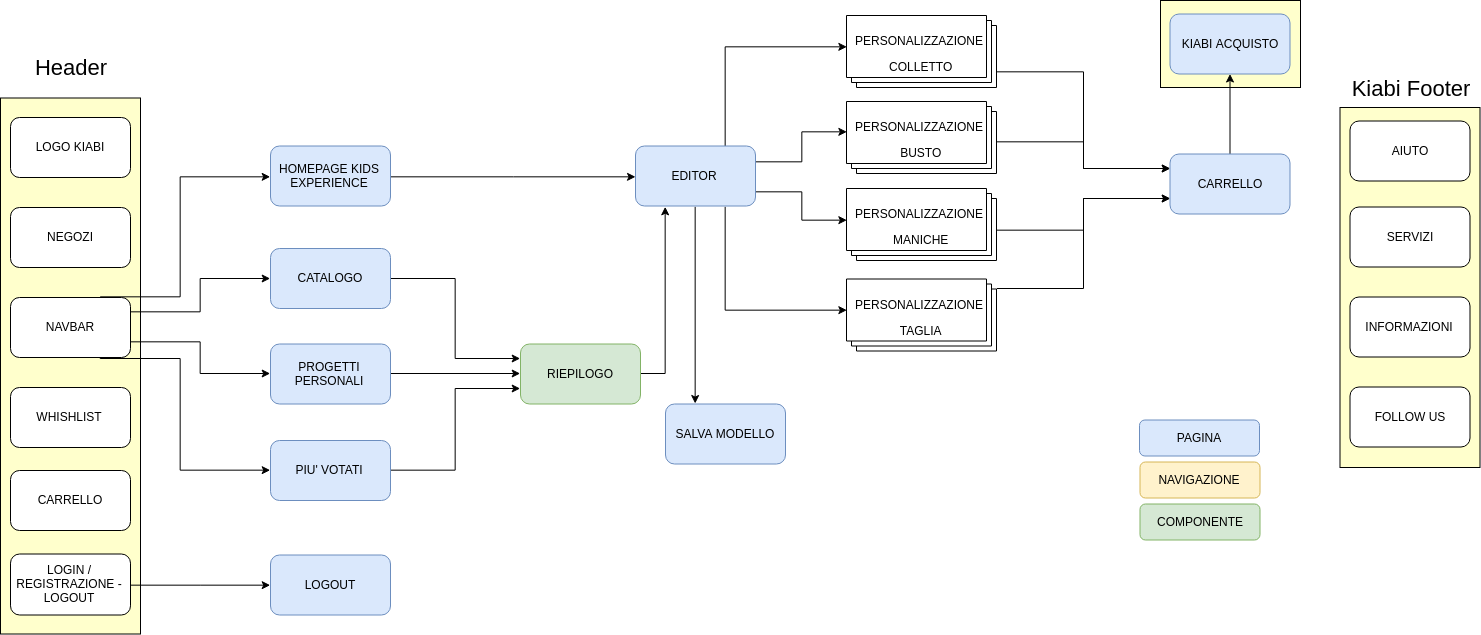
\includegraphics{blueprints/Creazione_modello.png}
\section{Wireframes}\label{Wireframes}
\subsection{Home} 
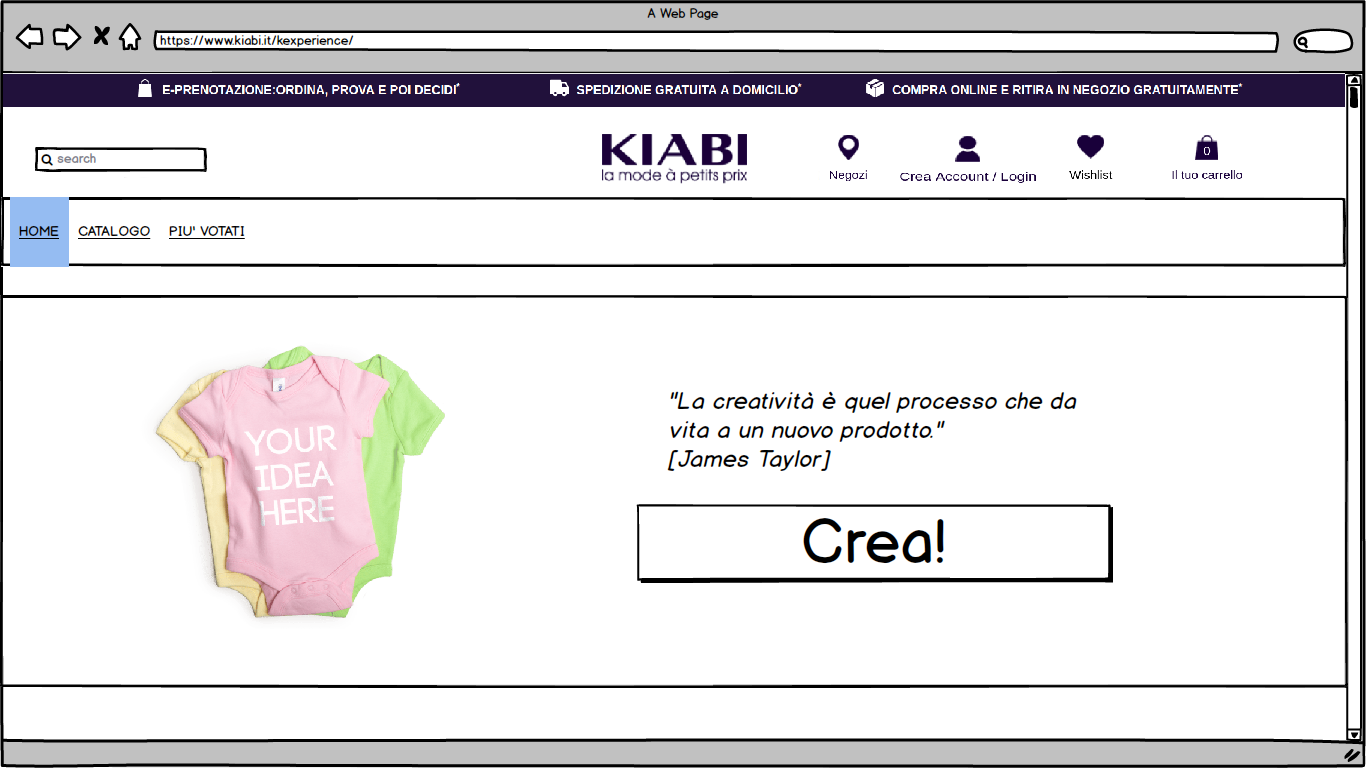
\includegraphics{balsamiq/Home Sottosito Utente Esterno .png}
\subsection{Catalogo} 
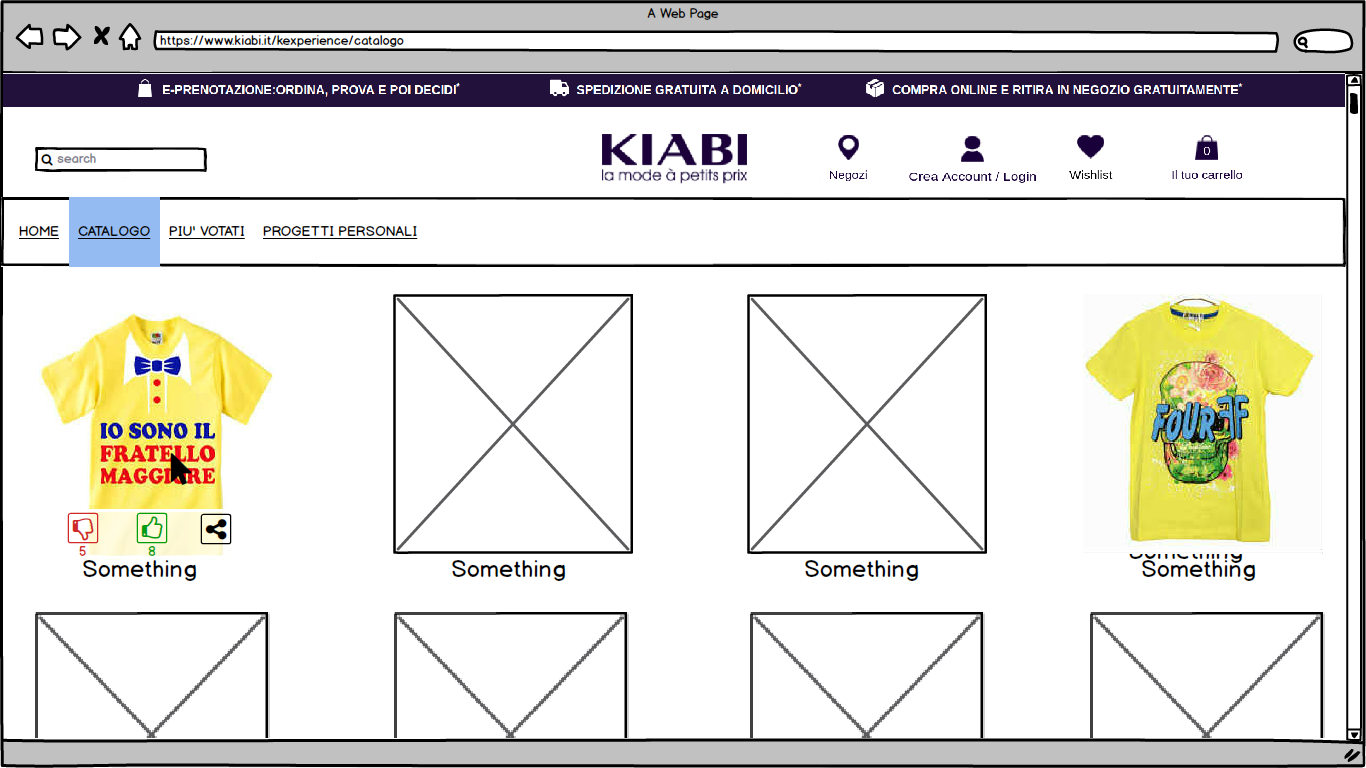
\includegraphics{balsamiq/Catalogo.png}
\subsubsection{Modifica Progetto Catalogo} 
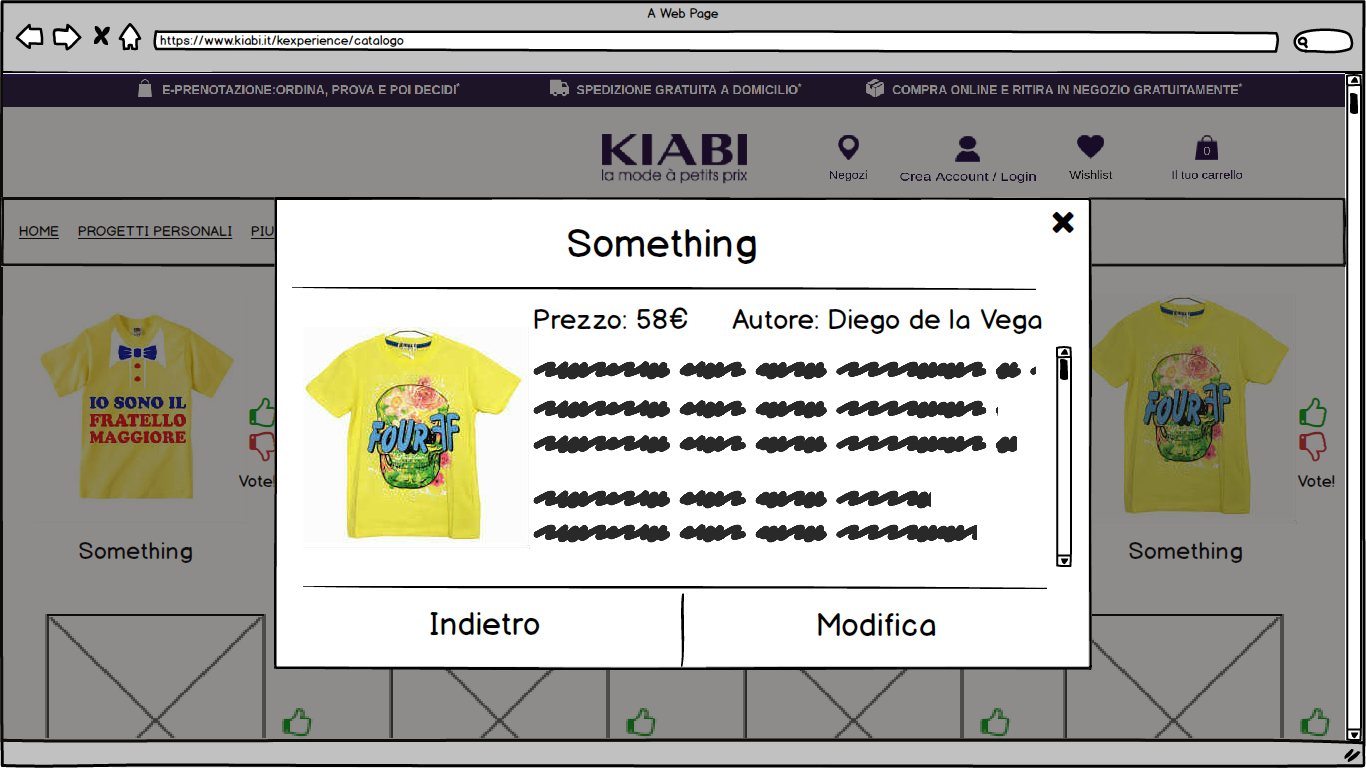
\includegraphics{balsamiq/Catalogo details.png}
\subsubsection{Votazione Progetto} 
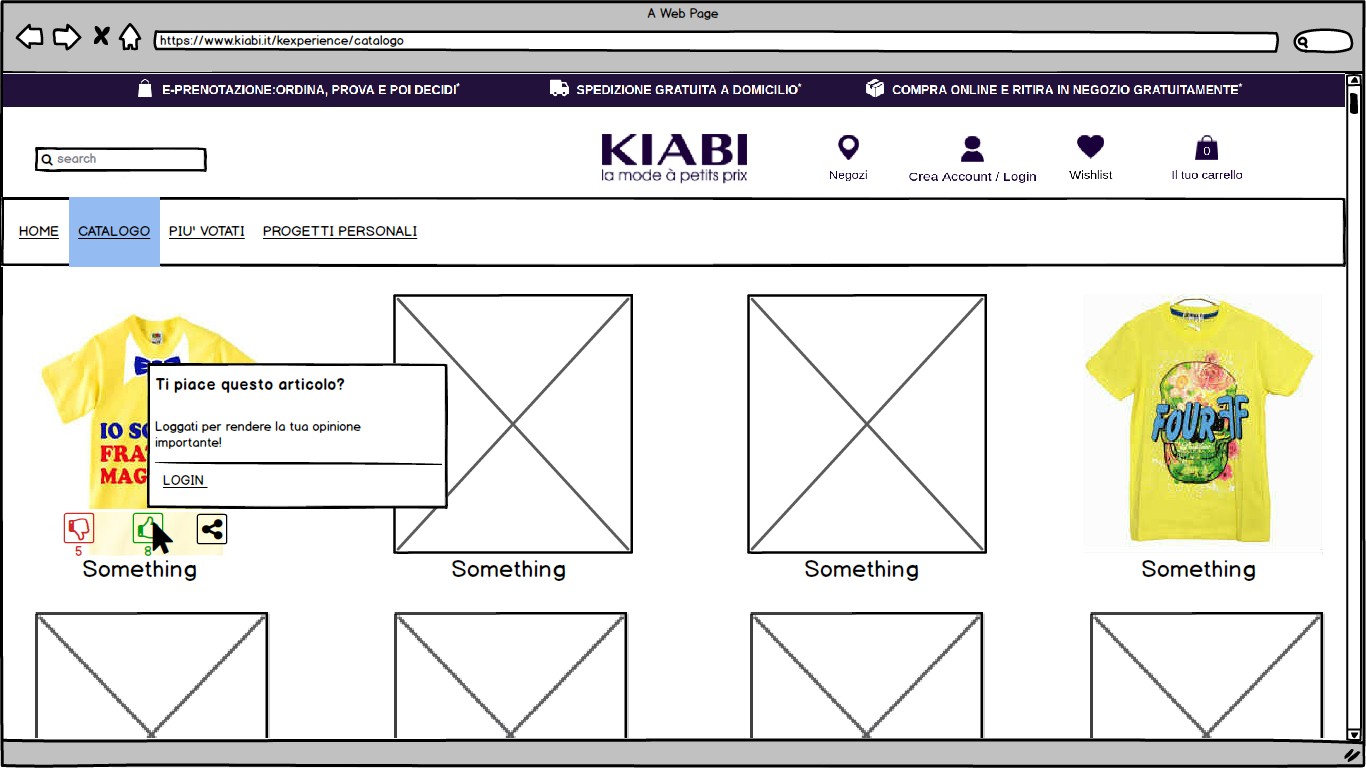
\includegraphics{balsamiq/Catalogo login.png}
\subsubsection{Login} 
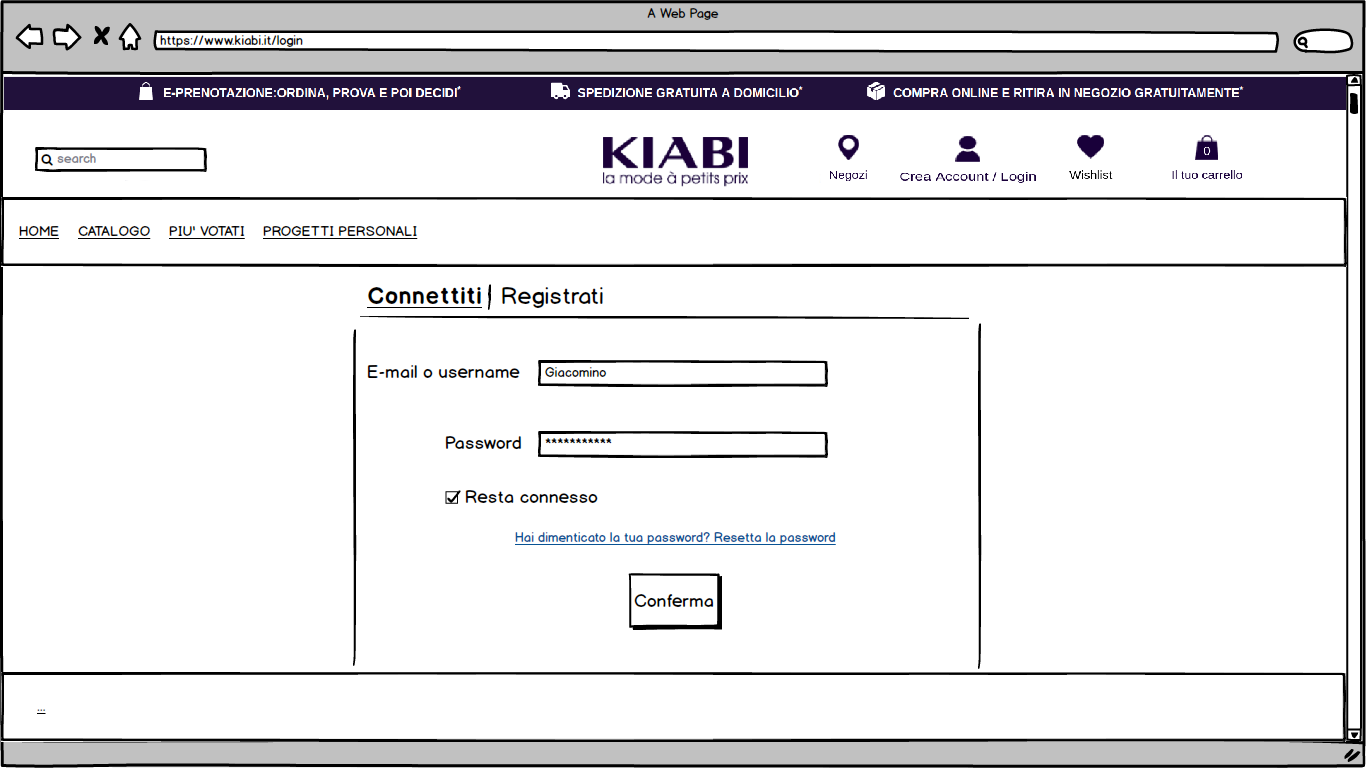
\includegraphics{balsamiq/Login.png}
\subsection{Progetti più votati} 
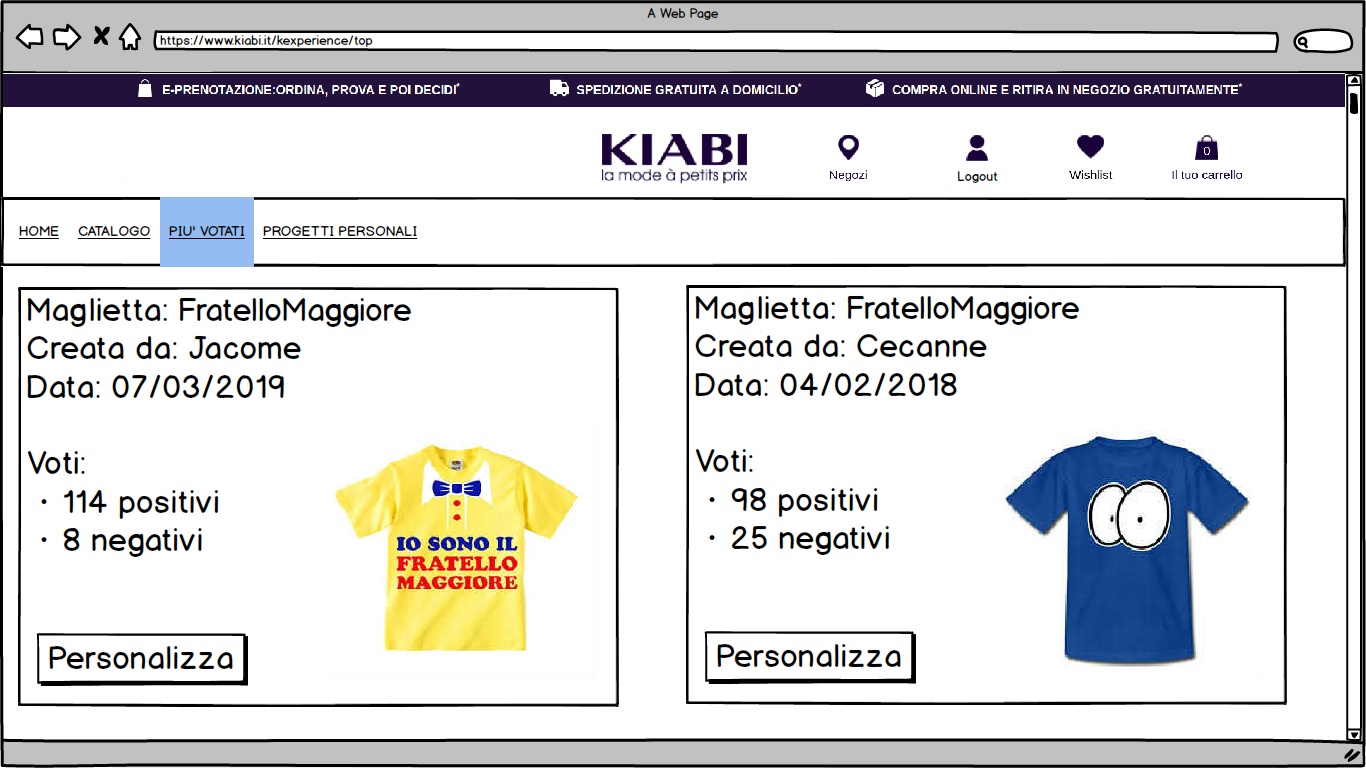
\includegraphics{balsamiq/Most Rated.png}
\subsection{Progetti Personali} 
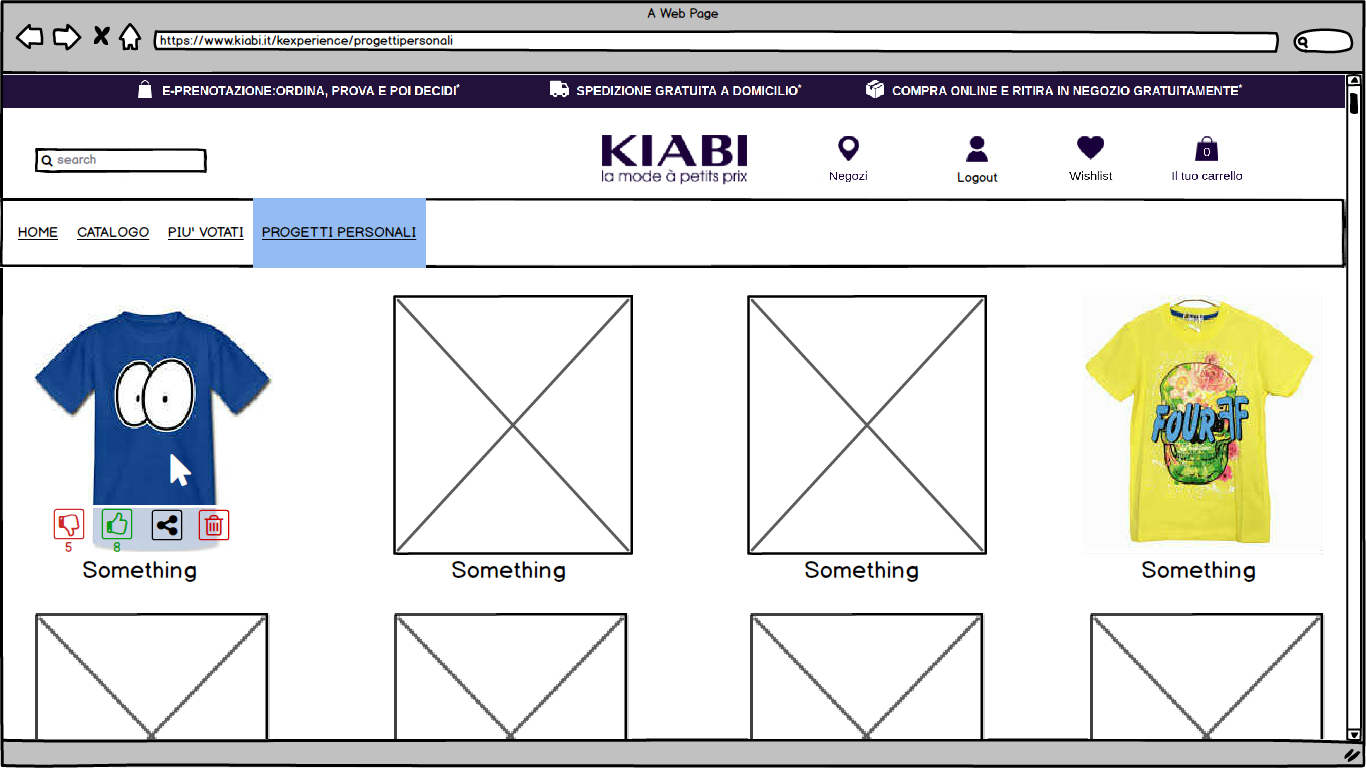
\includegraphics{balsamiq/Progetti Personali.png}
\subsubsection{Elimina Progetti Personali} 
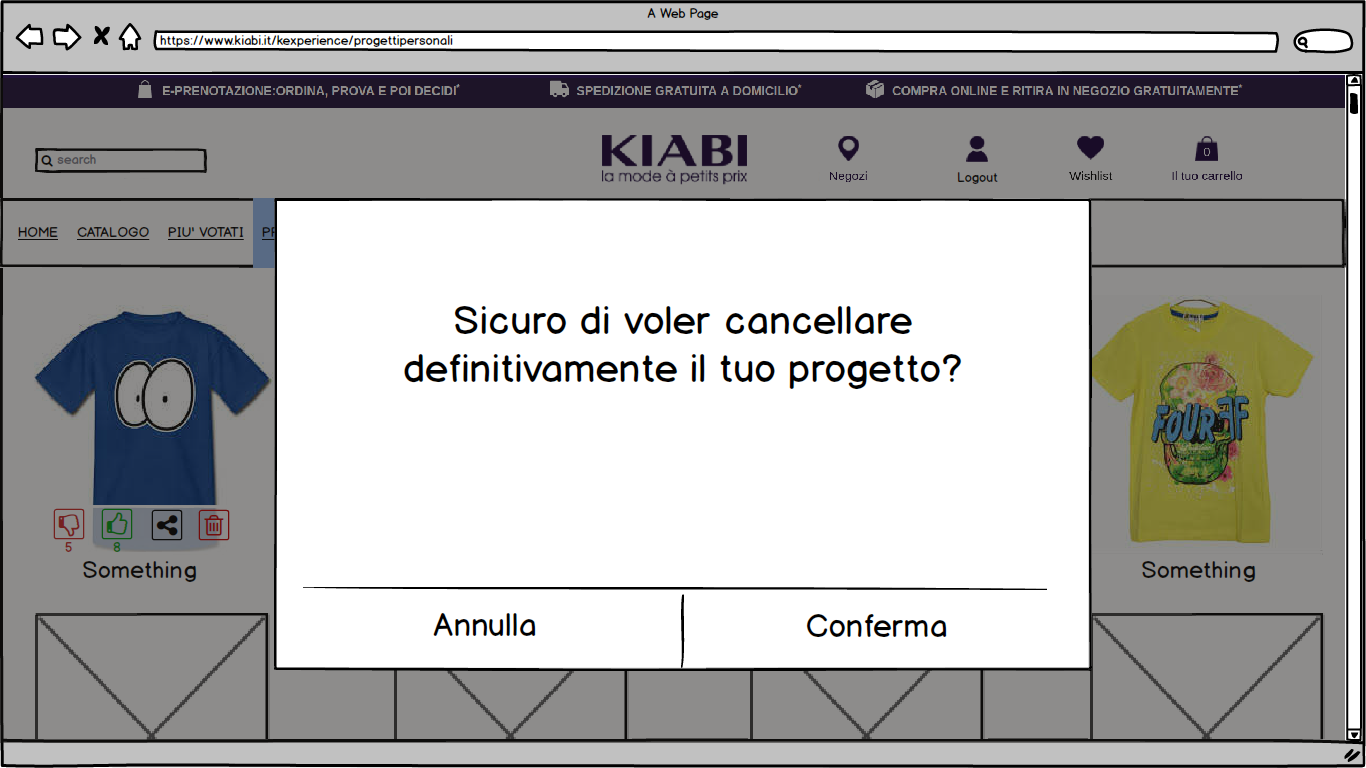
\includegraphics{balsamiq/Progetti Personali eliminazione.png}
\\
\\
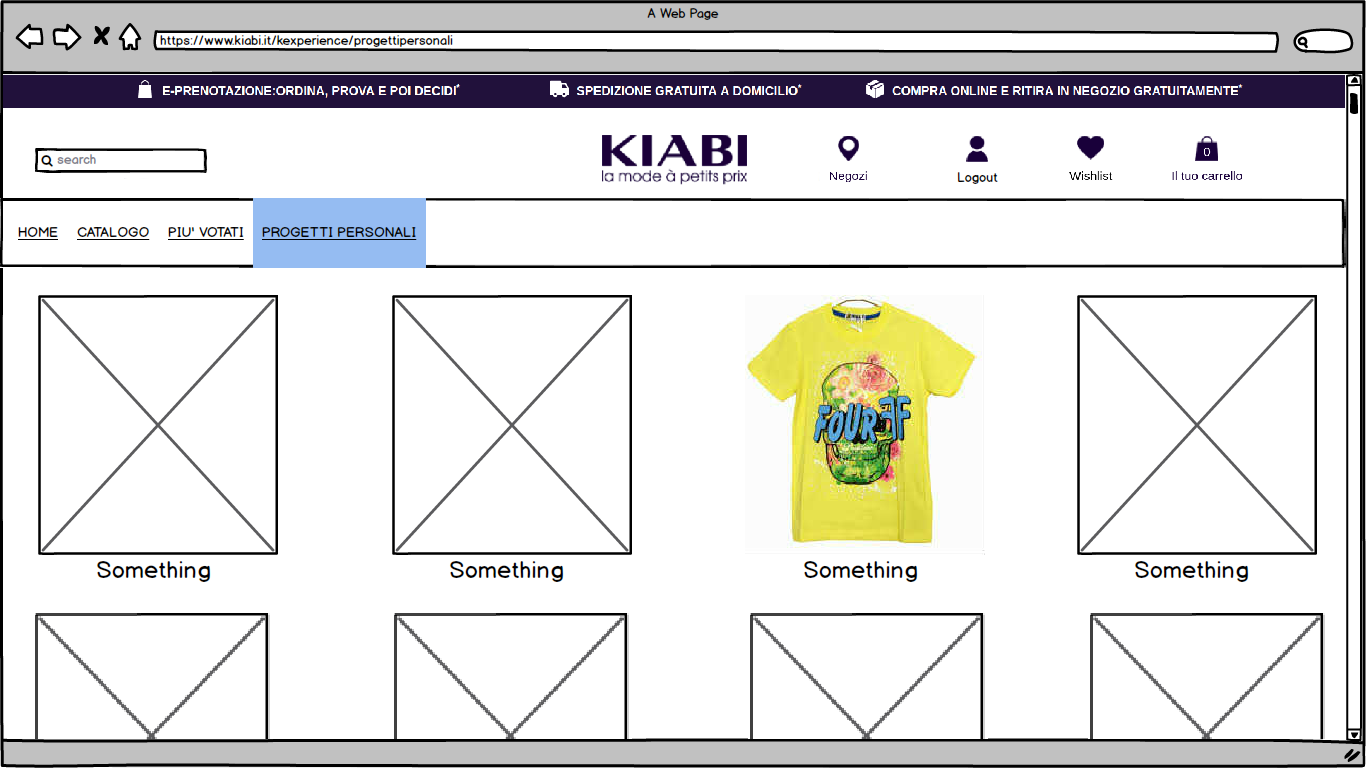
\includegraphics{balsamiq/Progetti Personali eliminazione post eliminazione.png}
\subsection{Editor} 
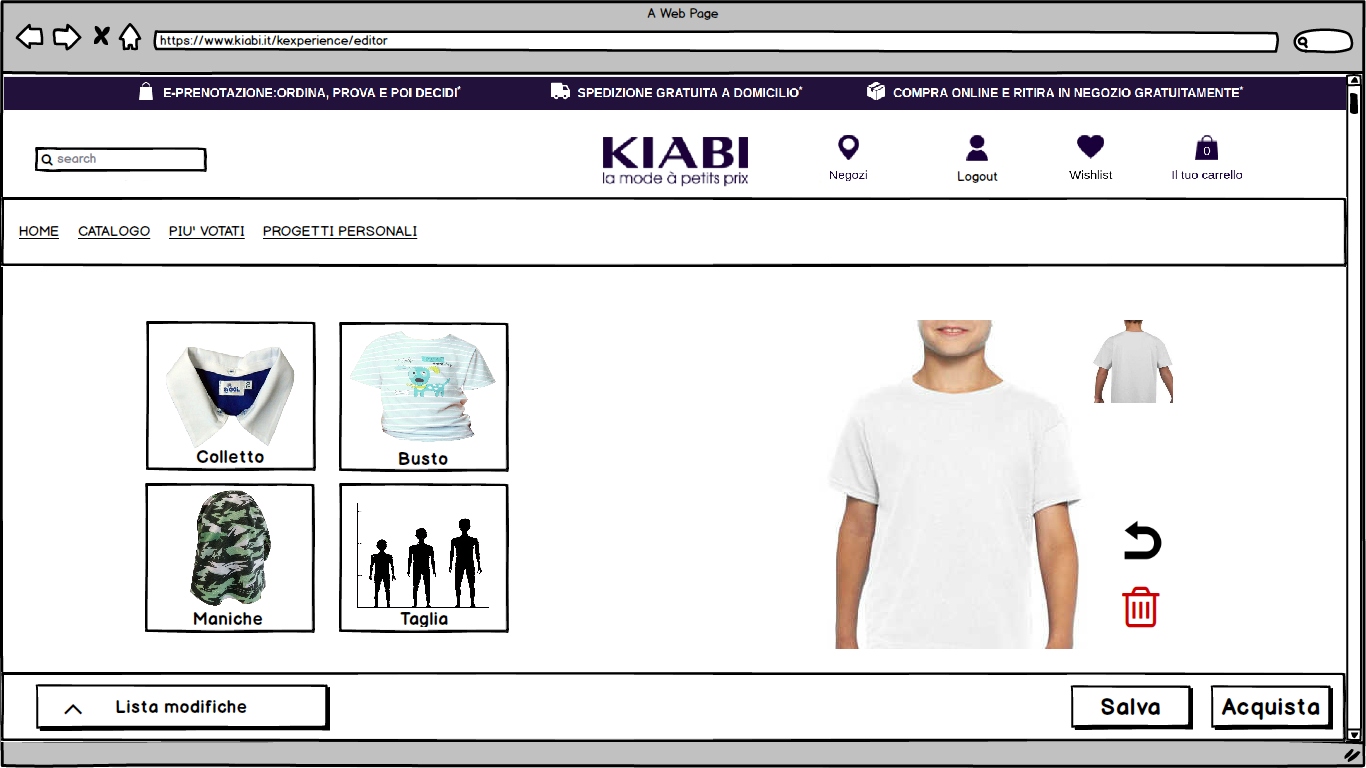
\includegraphics{balsamiq/Editor base.png}
\subsubsection{Salvataggio Progetto} 
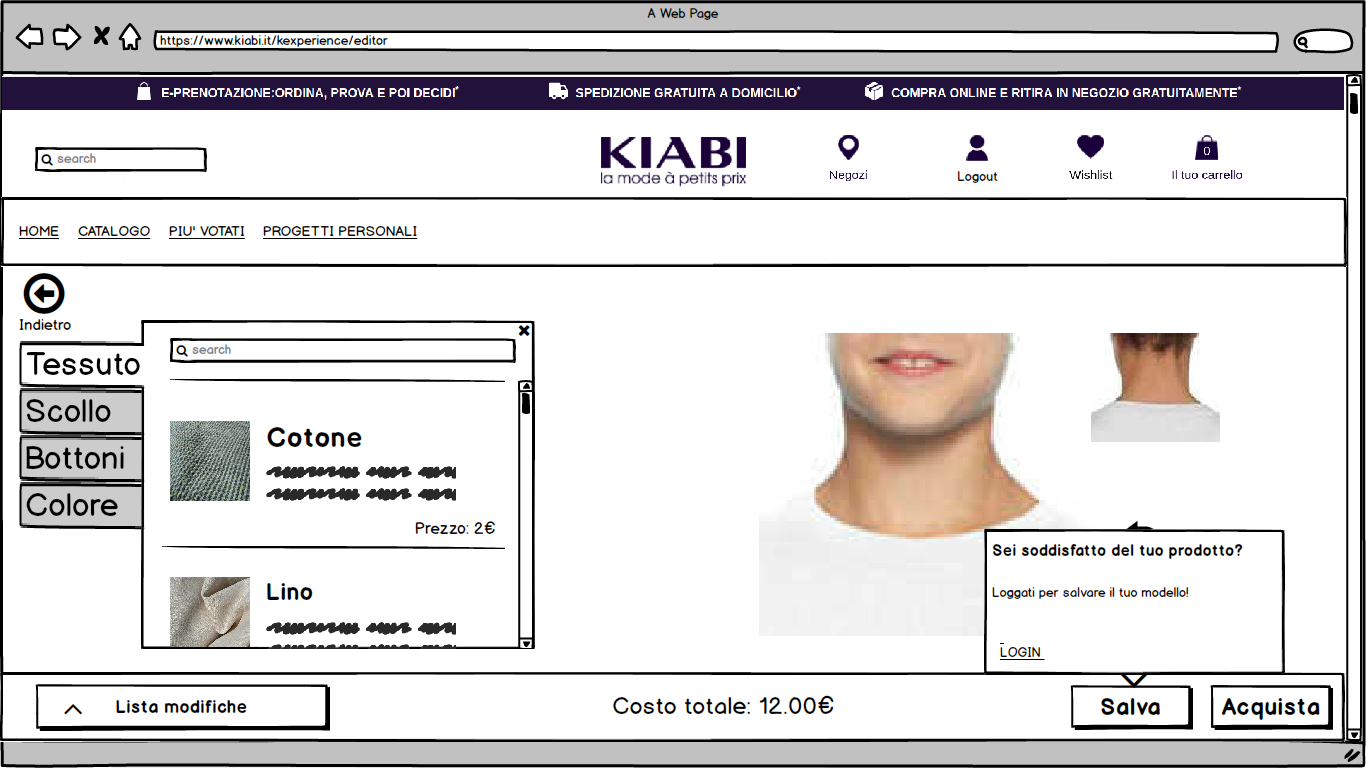
\includegraphics{balsamiq/Editor - caratteristica collo tessuto non loggato.png}
\subsubsection{Editor Colletto} 
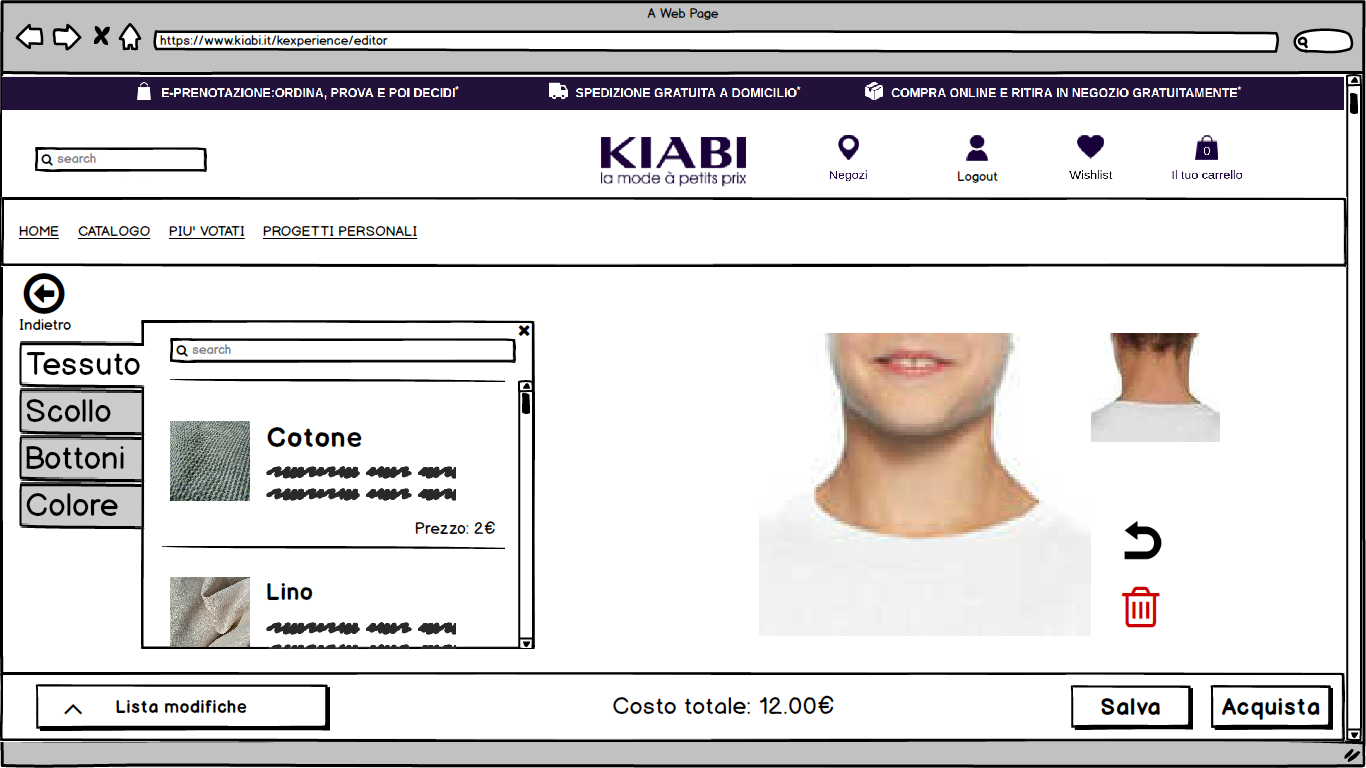
\includegraphics{balsamiq/Editor - caratteristica collo tessuto.png}
\\
\\
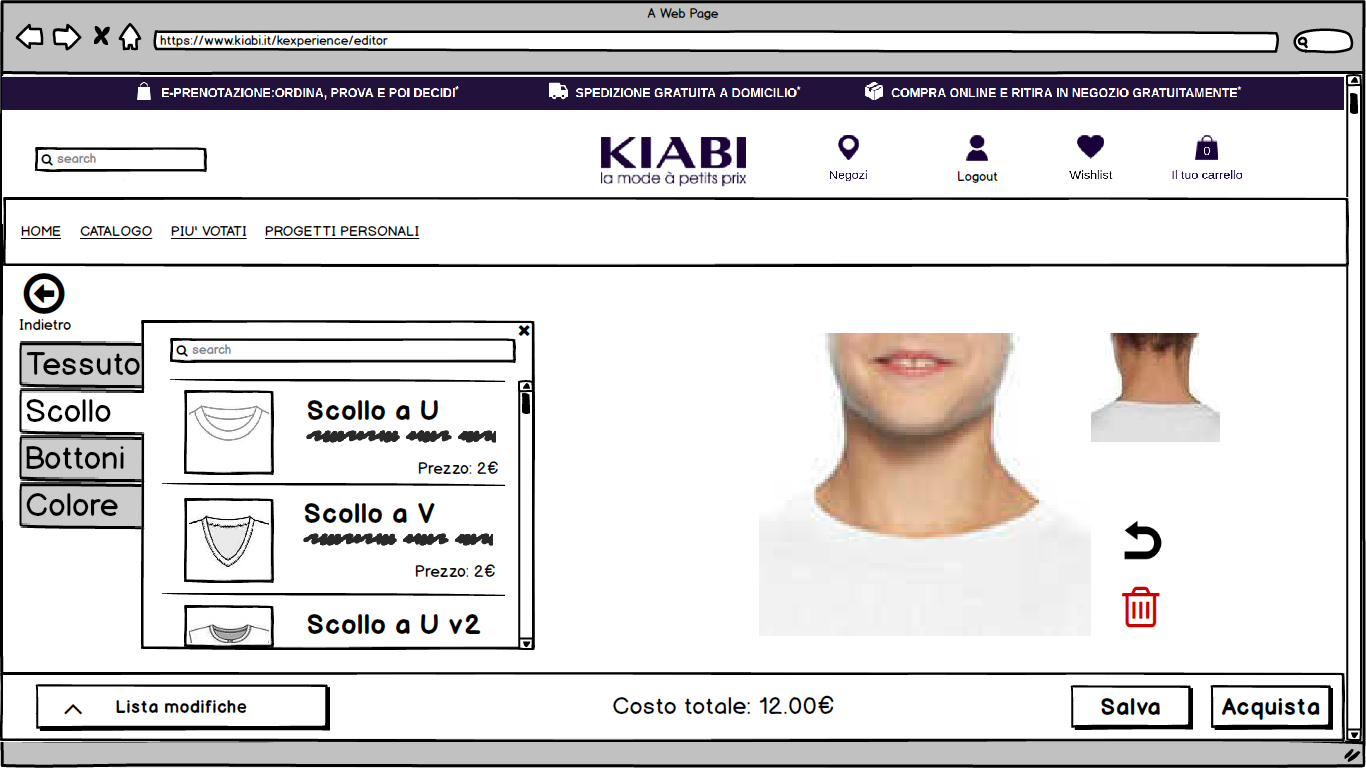
\includegraphics{balsamiq/Editor - caratteristica collo scollo.png}
\\
\\
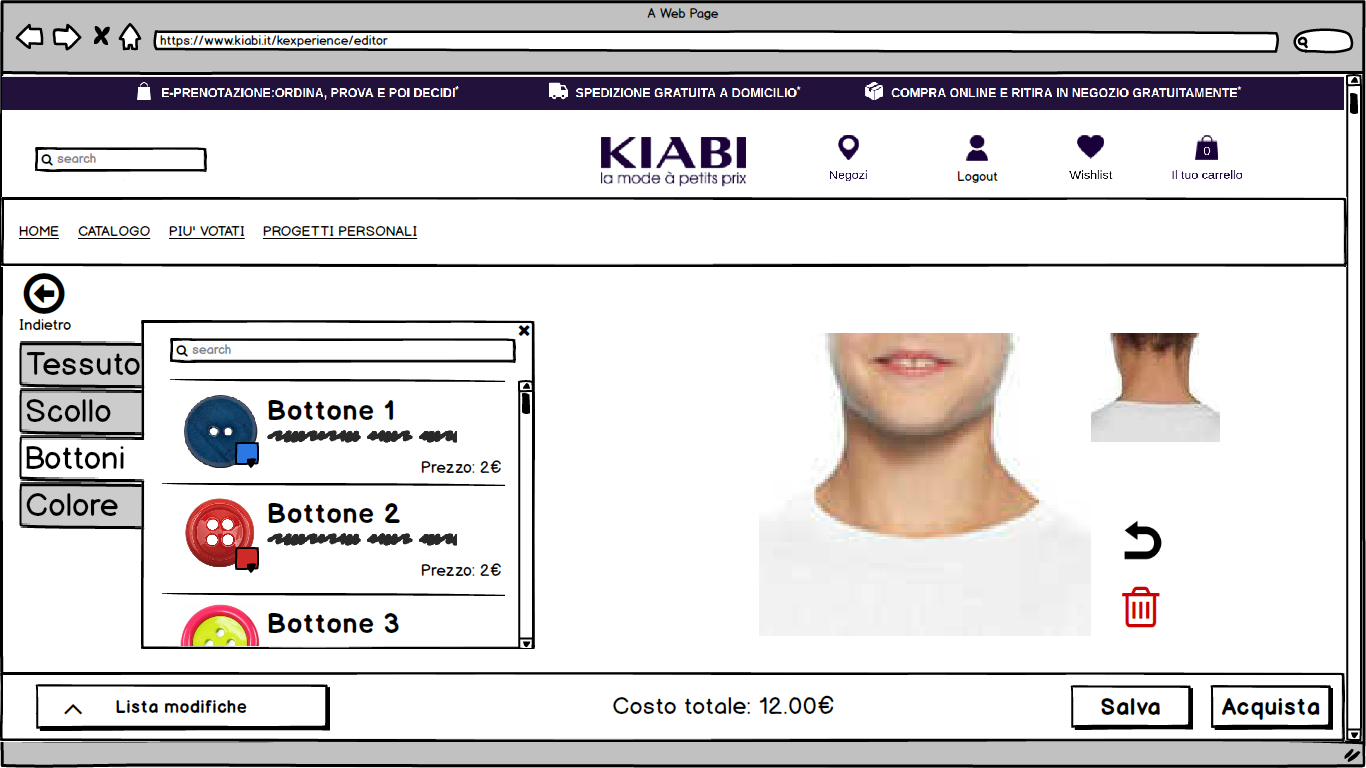
\includegraphics{balsamiq/Editor - caratteristica collo bottoni.png}
\\
\\
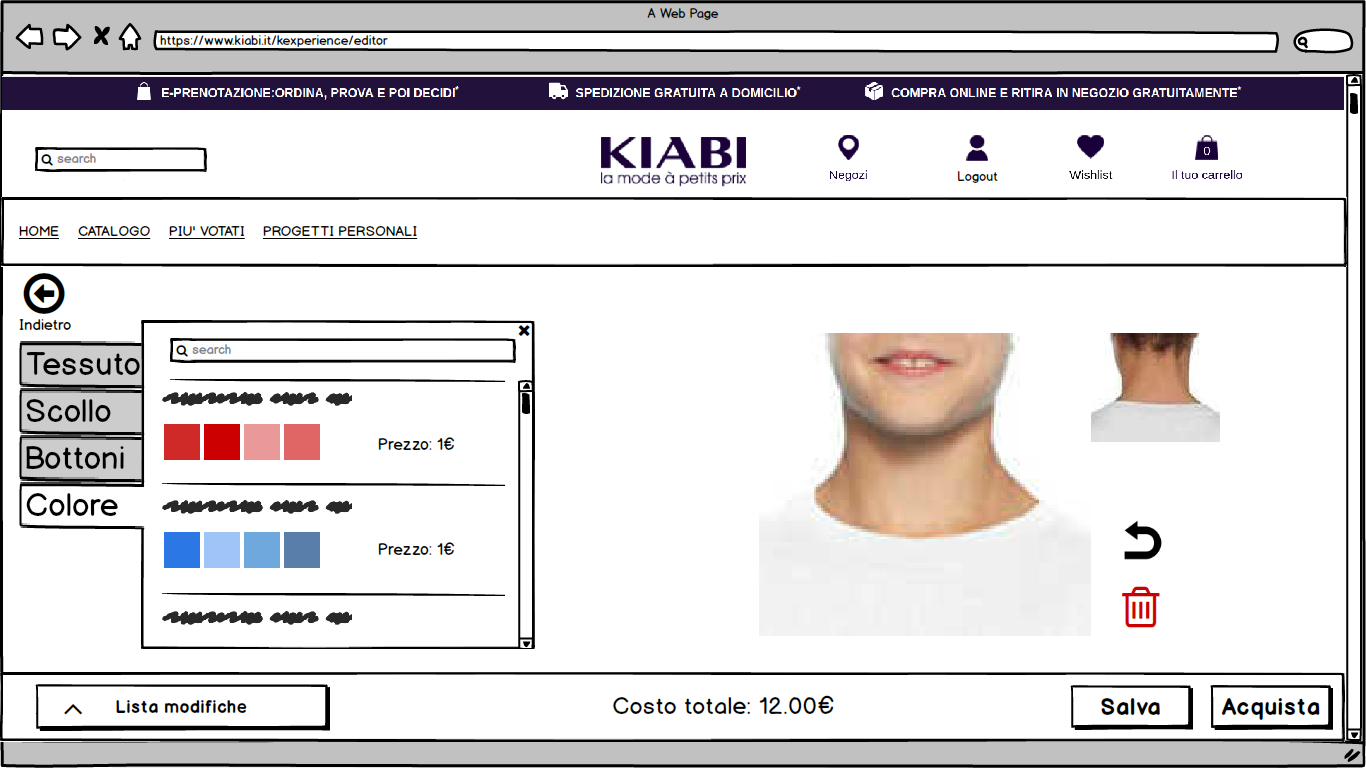
\includegraphics{balsamiq/Editor - caratteristica collo colore.png}
\subsubsection{Editor Busto} 
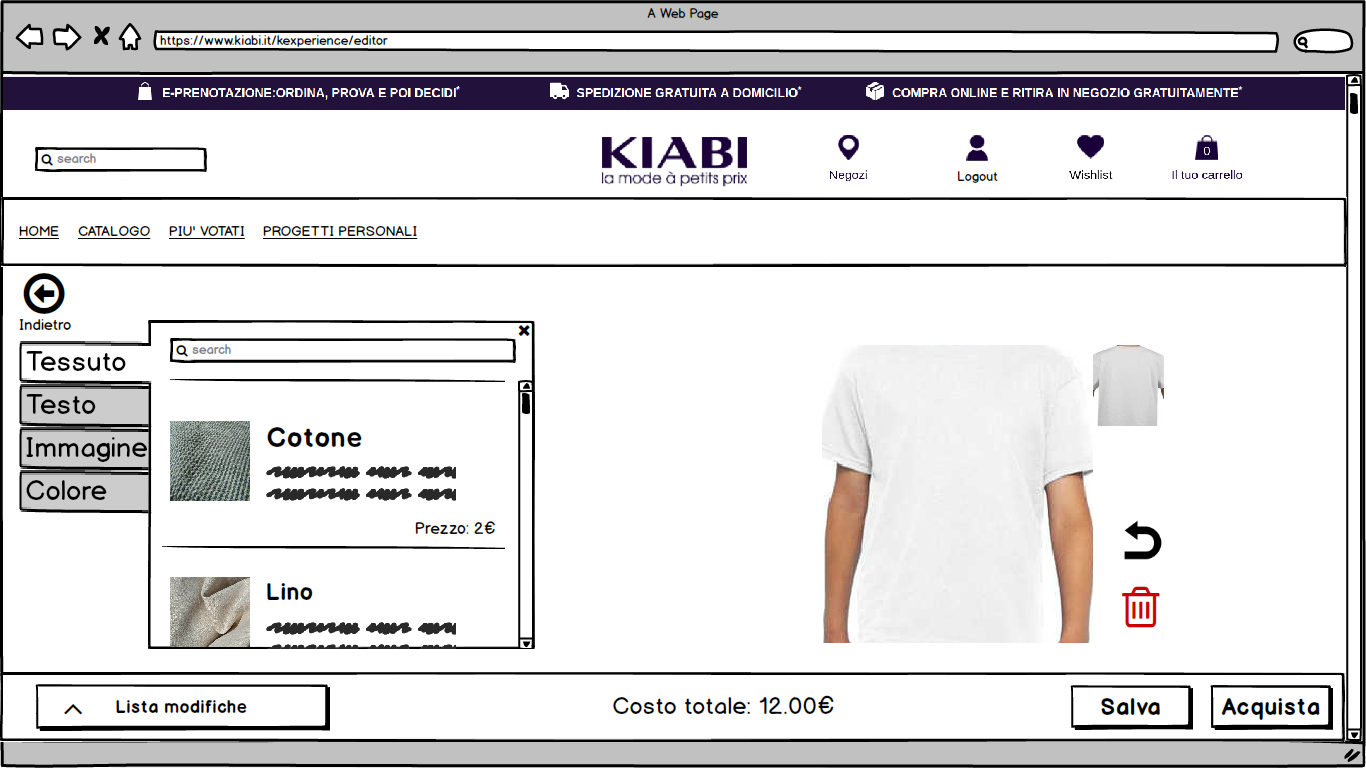
\includegraphics{balsamiq/Editor - caratteristica busto tessuto.png}
\\
\\
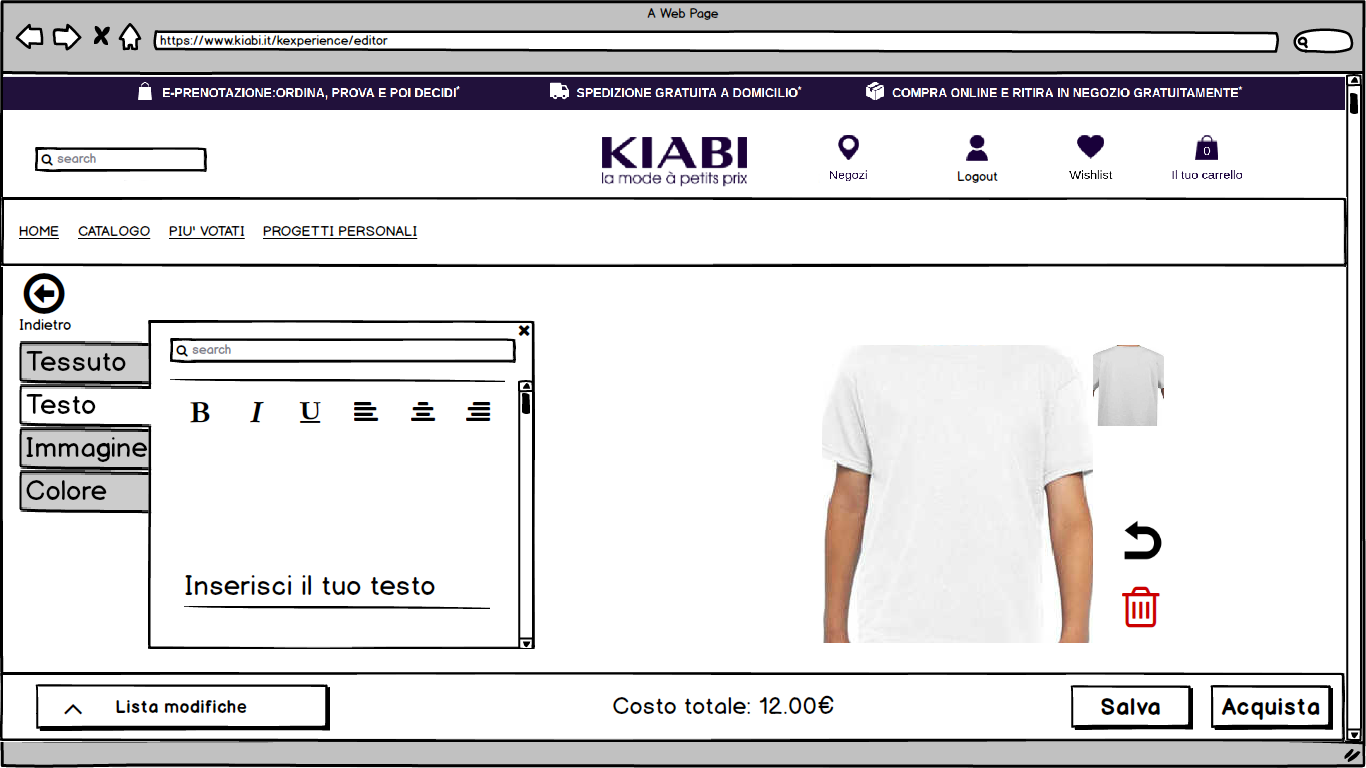
\includegraphics{balsamiq/Editor - caratteristica busto testo.png}
\\
\\
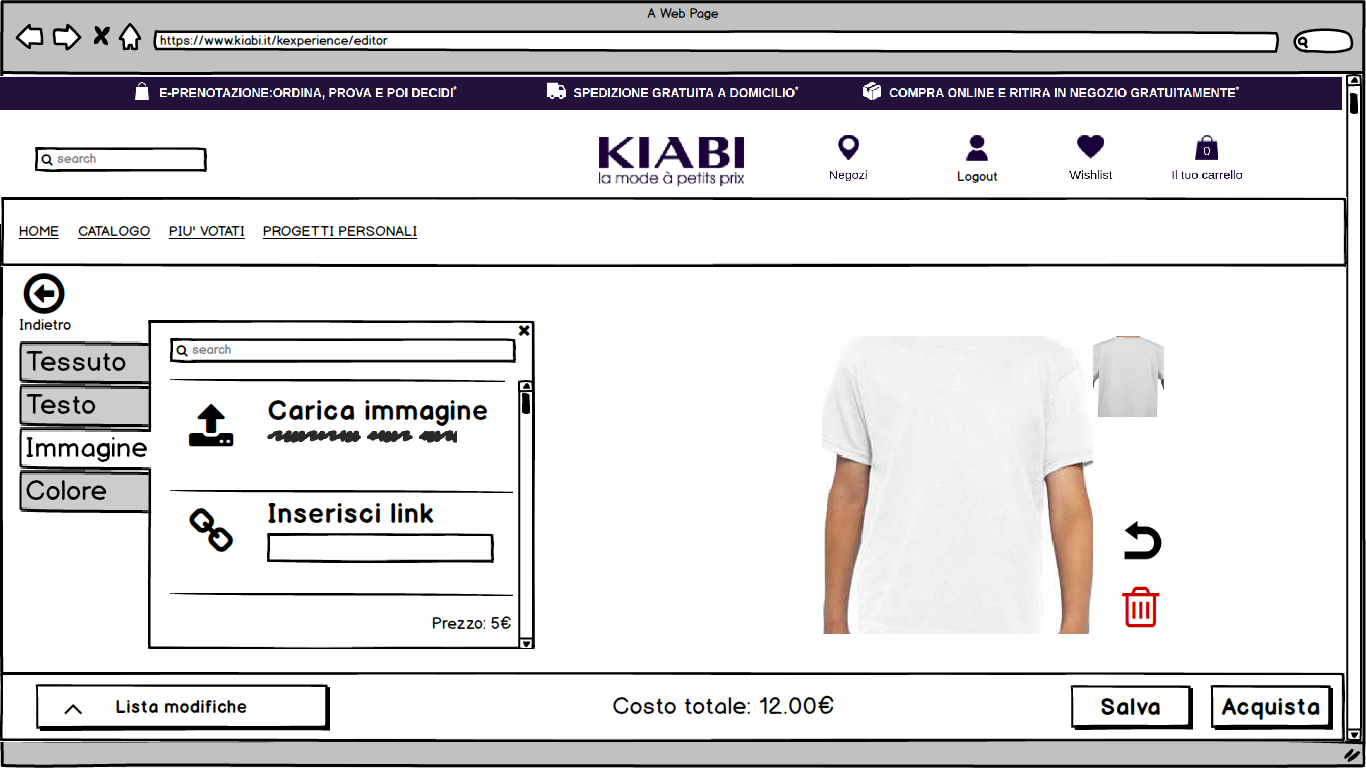
\includegraphics{balsamiq/Editor - caratteristica busto immagine.png}
\\
\\
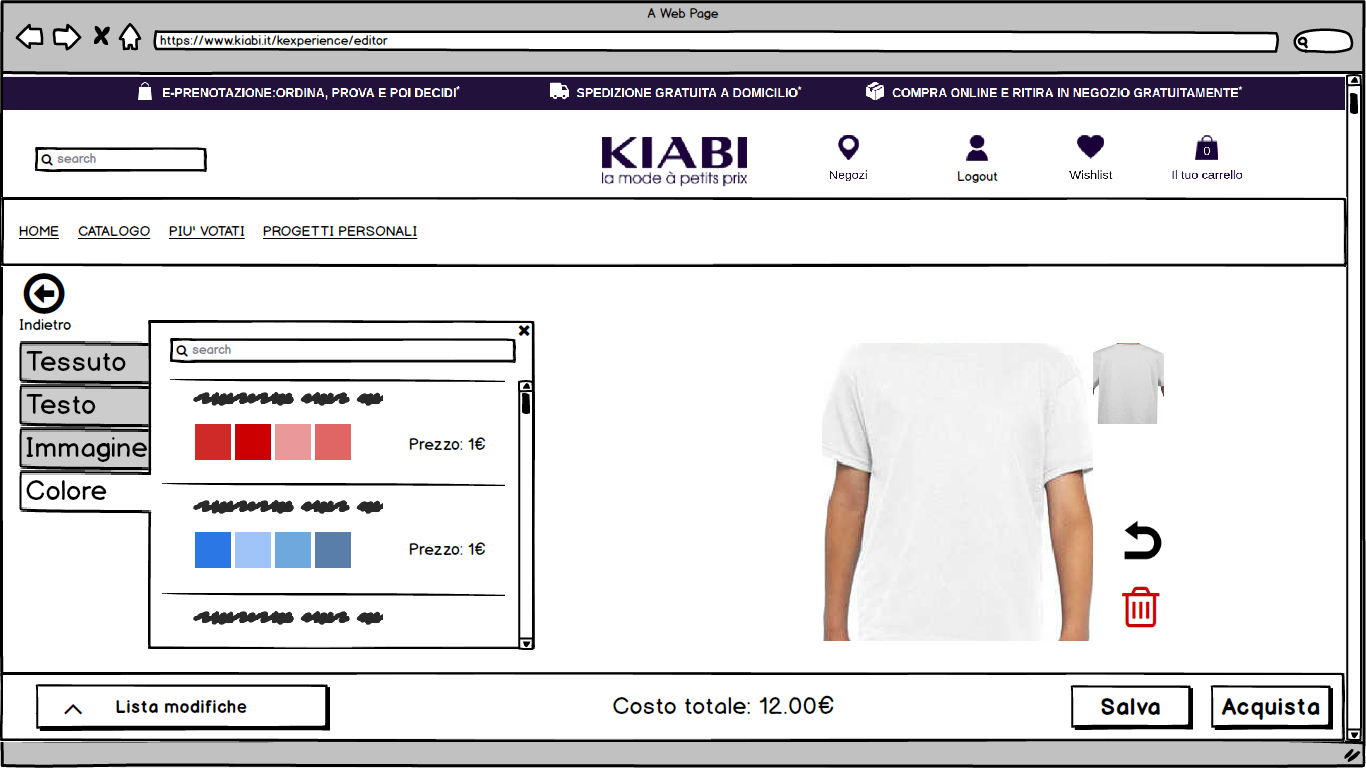
\includegraphics{balsamiq/Editor - caratteristica busto colore.png}
\subsubsection{Editor Maniche} 
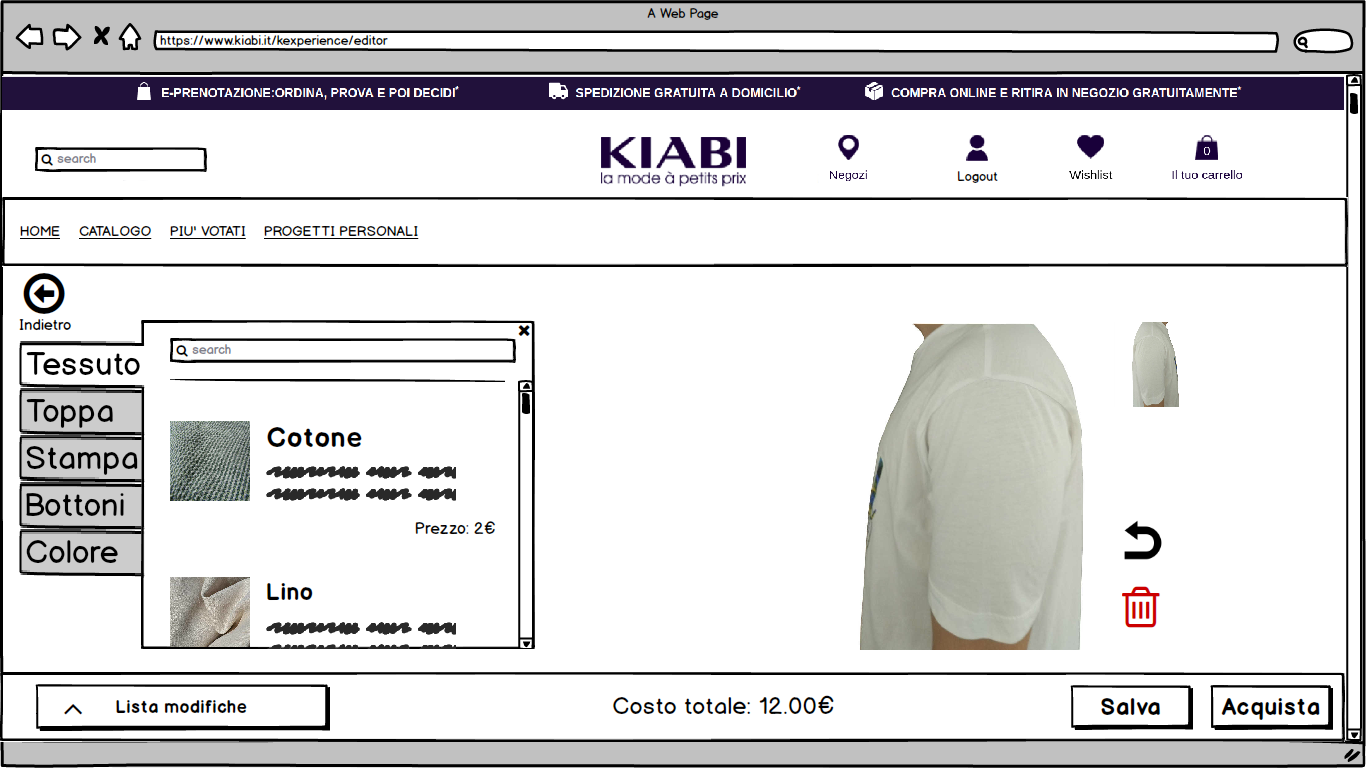
\includegraphics{balsamiq/Editor - caratteristica maniche tessuto.png}
\\
\\
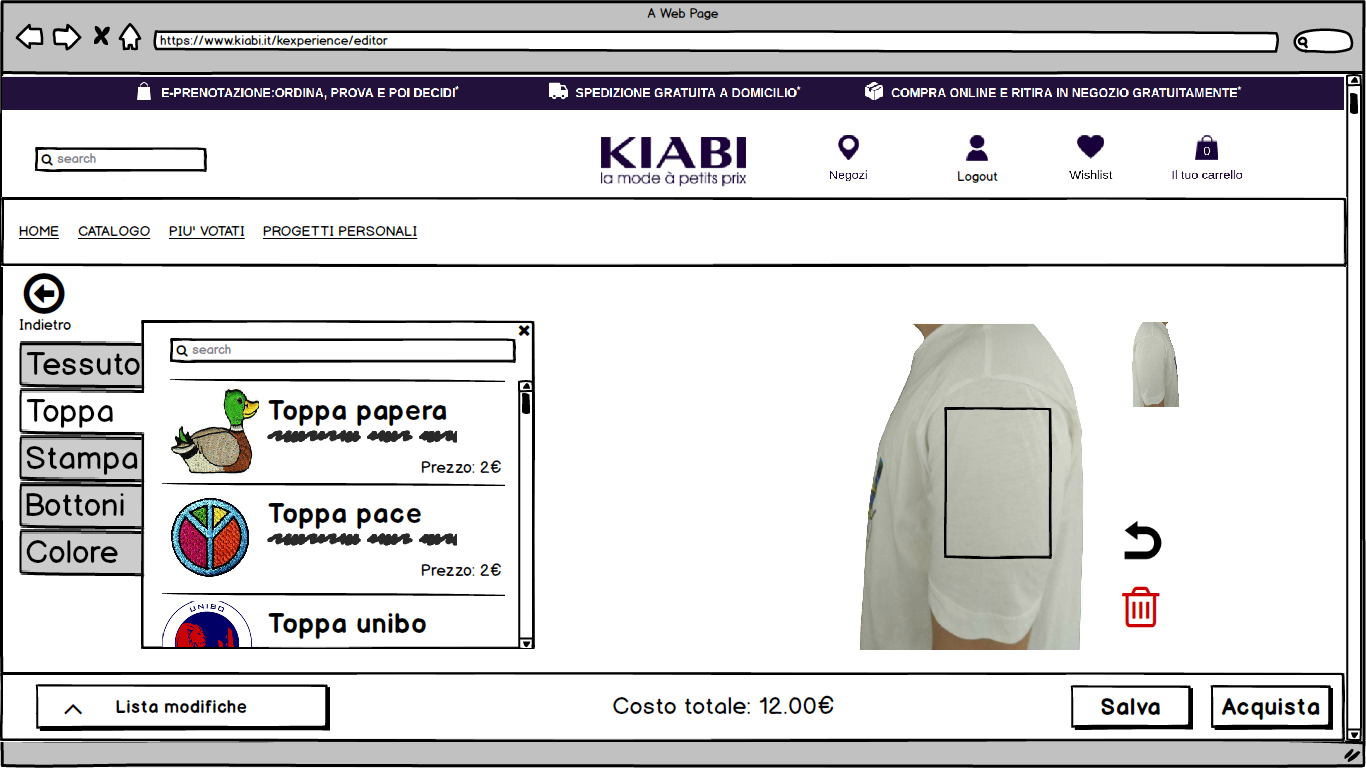
\includegraphics{balsamiq/Editor - caratteristica maniche toppa.png}
\\
\\
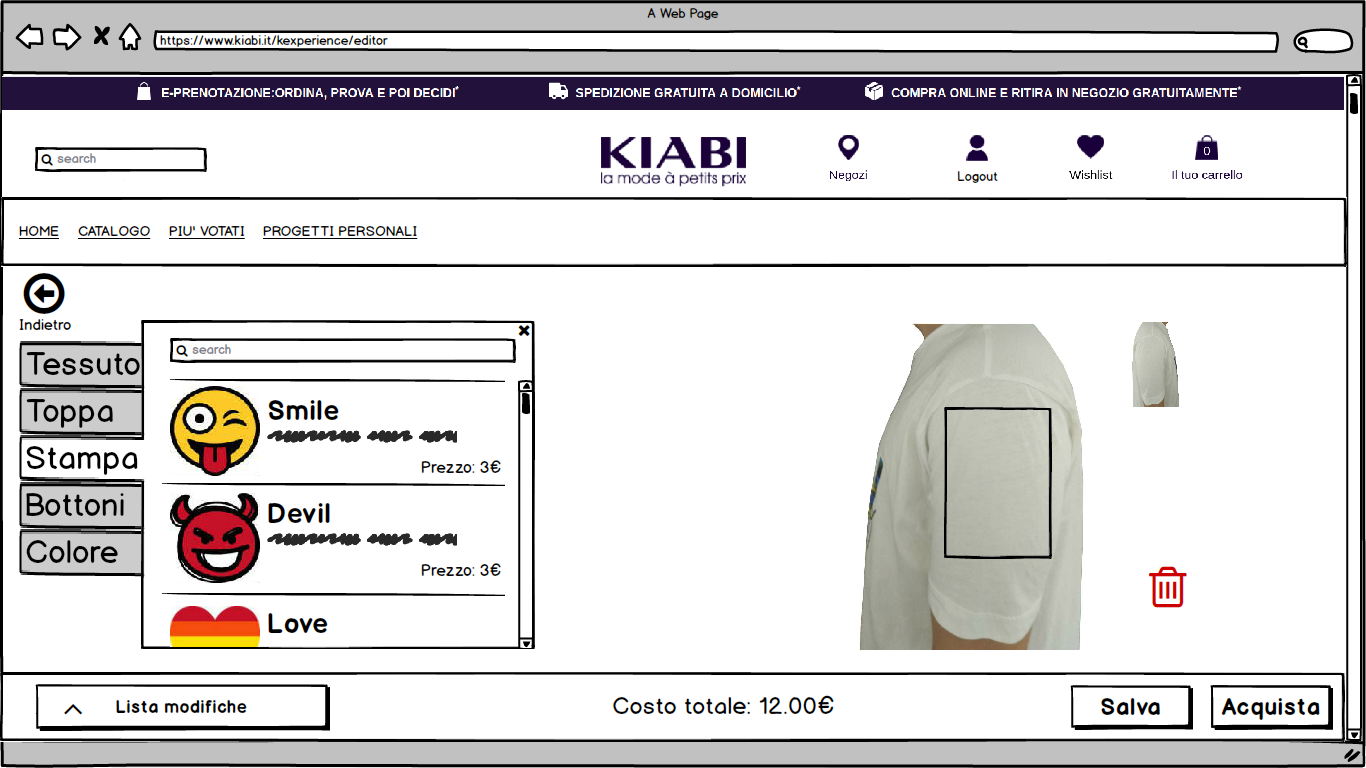
\includegraphics{balsamiq/Editor - caratteristica maniche stampa.png}
\\
\\
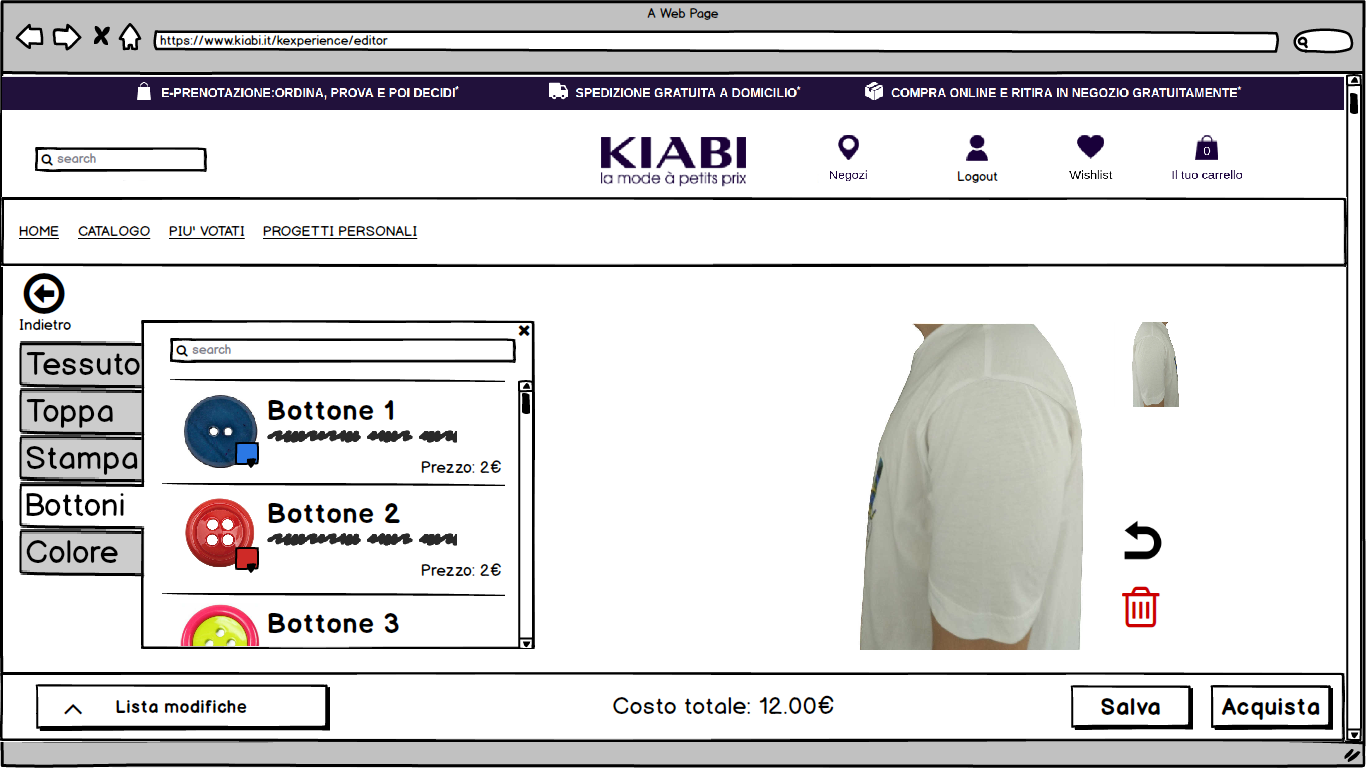
\includegraphics{balsamiq/Editor - caratteristica maniche bottoni.png}
\\
\\
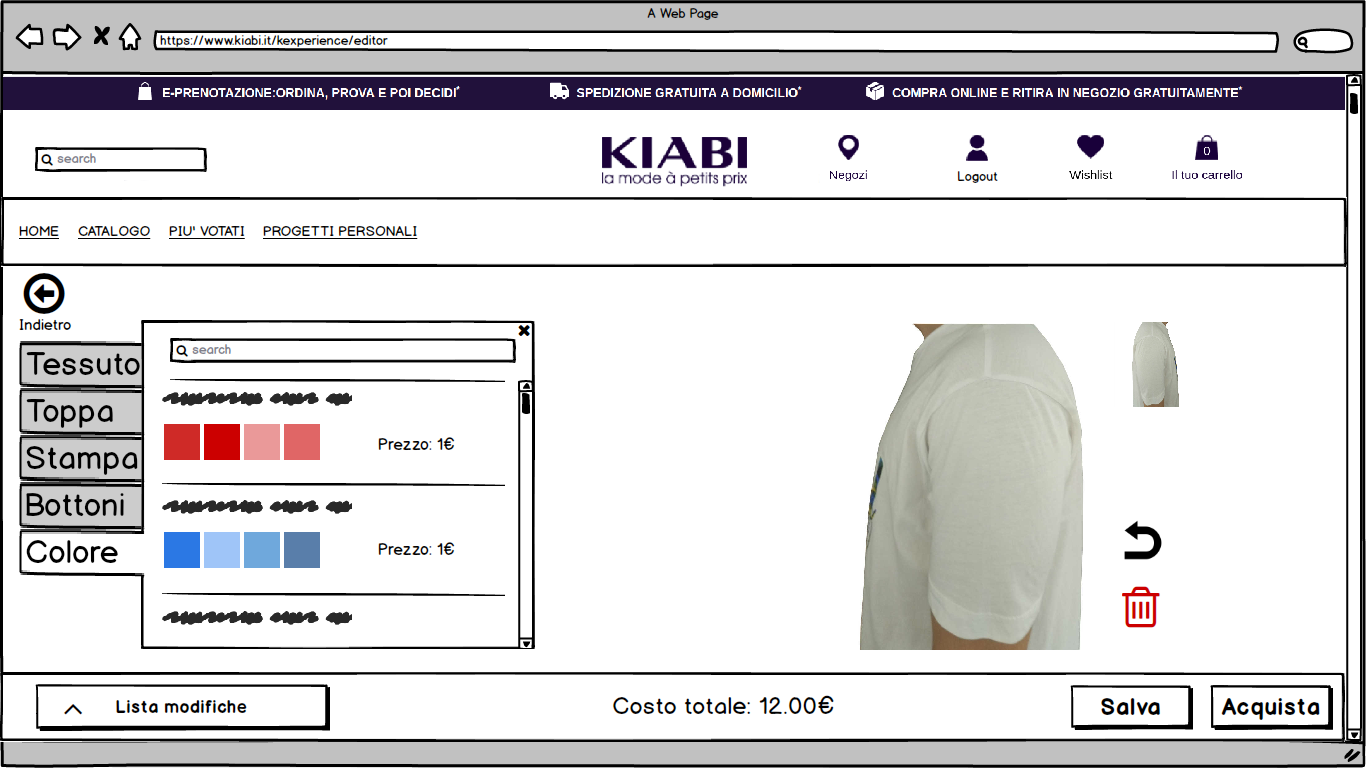
\includegraphics{balsamiq/Editor - caratteristica maniche colore.png}
\subsubsection{Taglia} 
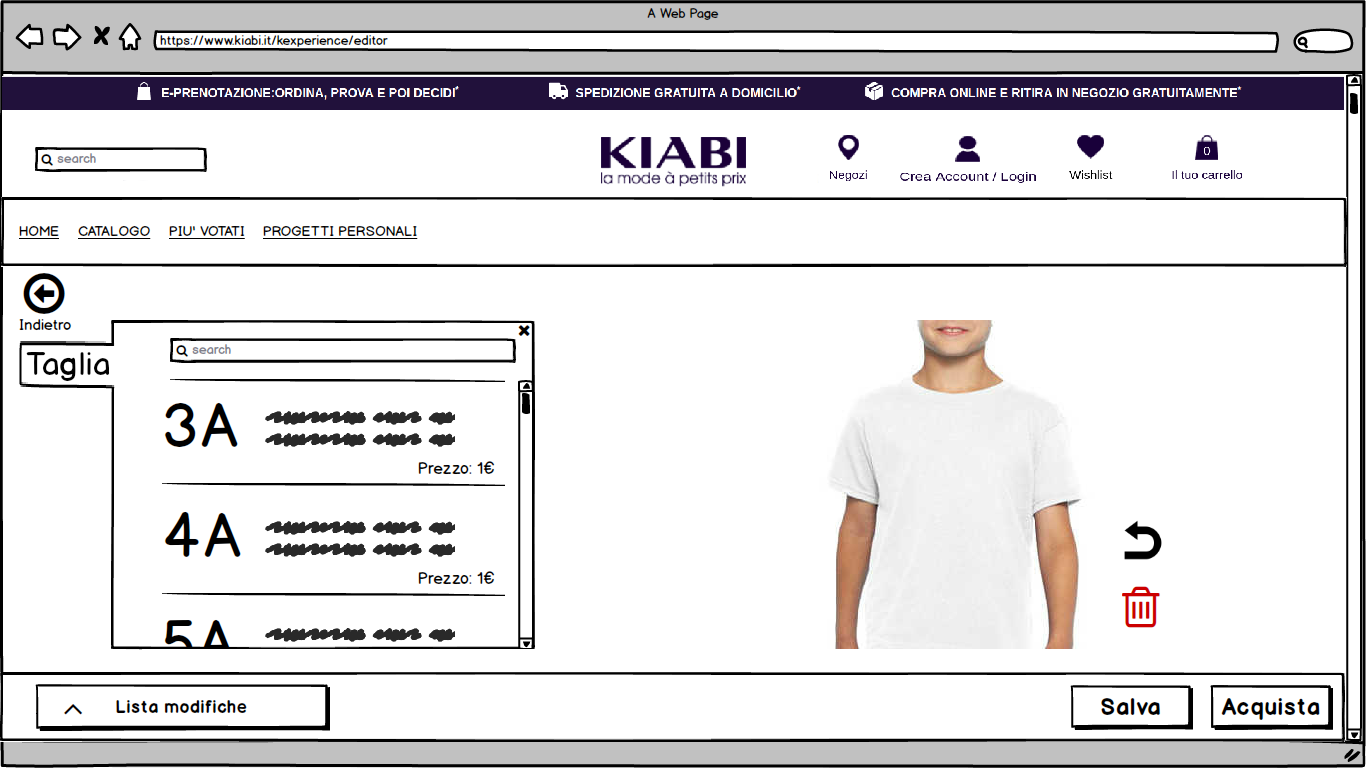
\includegraphics{balsamiq/Editor - caratteristica capo taglia.png}
\subsubsection{Lista Dettagli} 
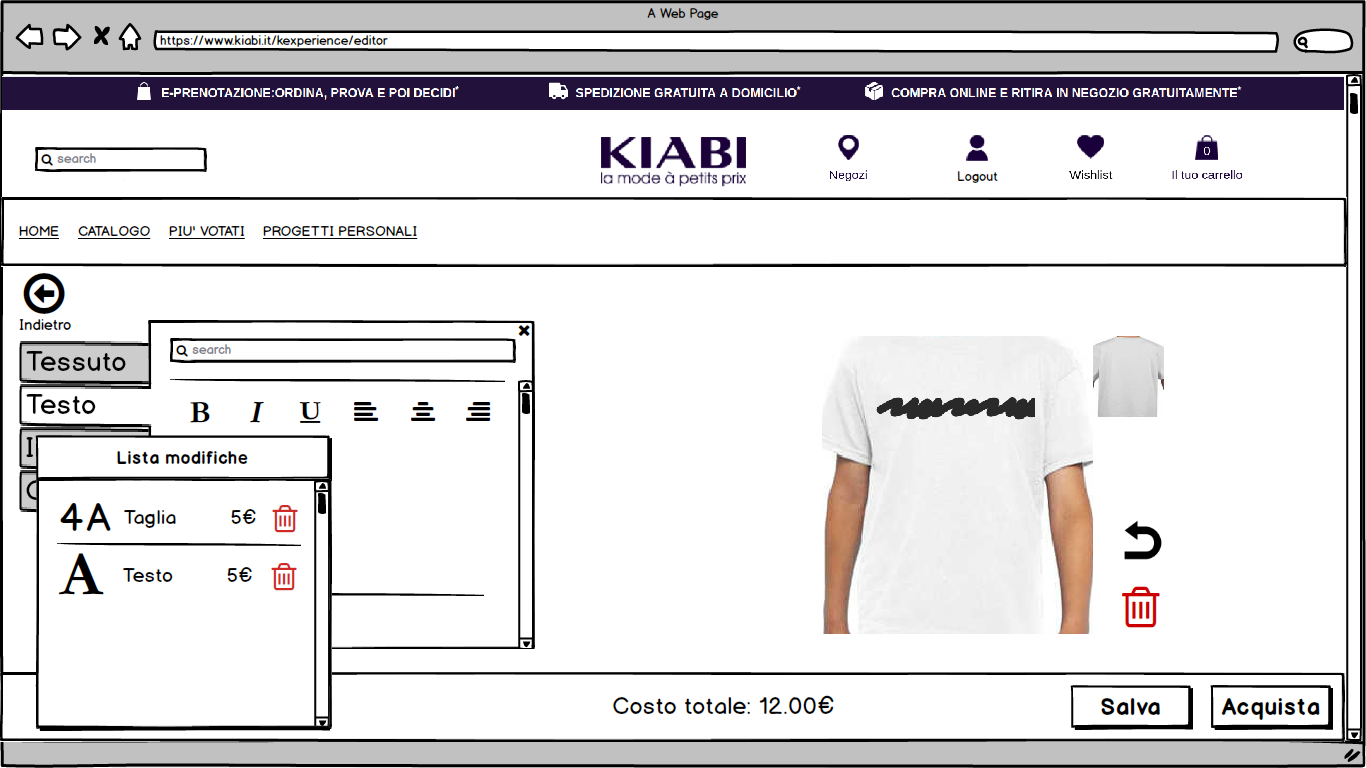
\includegraphics{balsamiq/Editor - caratteristica busto testo 4.png}
\subsection{Carrello} 
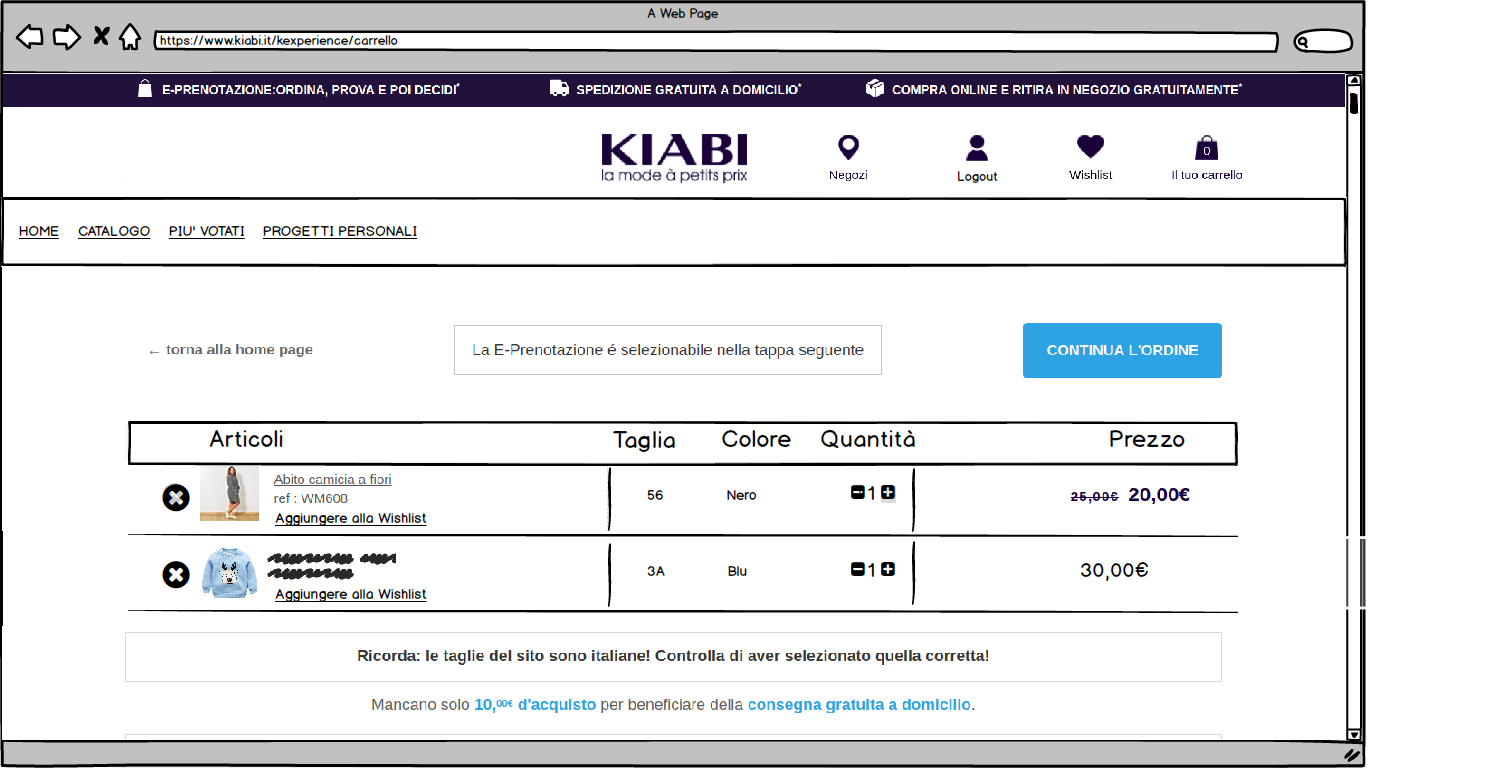
\includegraphics{balsamiq/Carrello.png}
\subsubsection{Dettagli Carrello} 
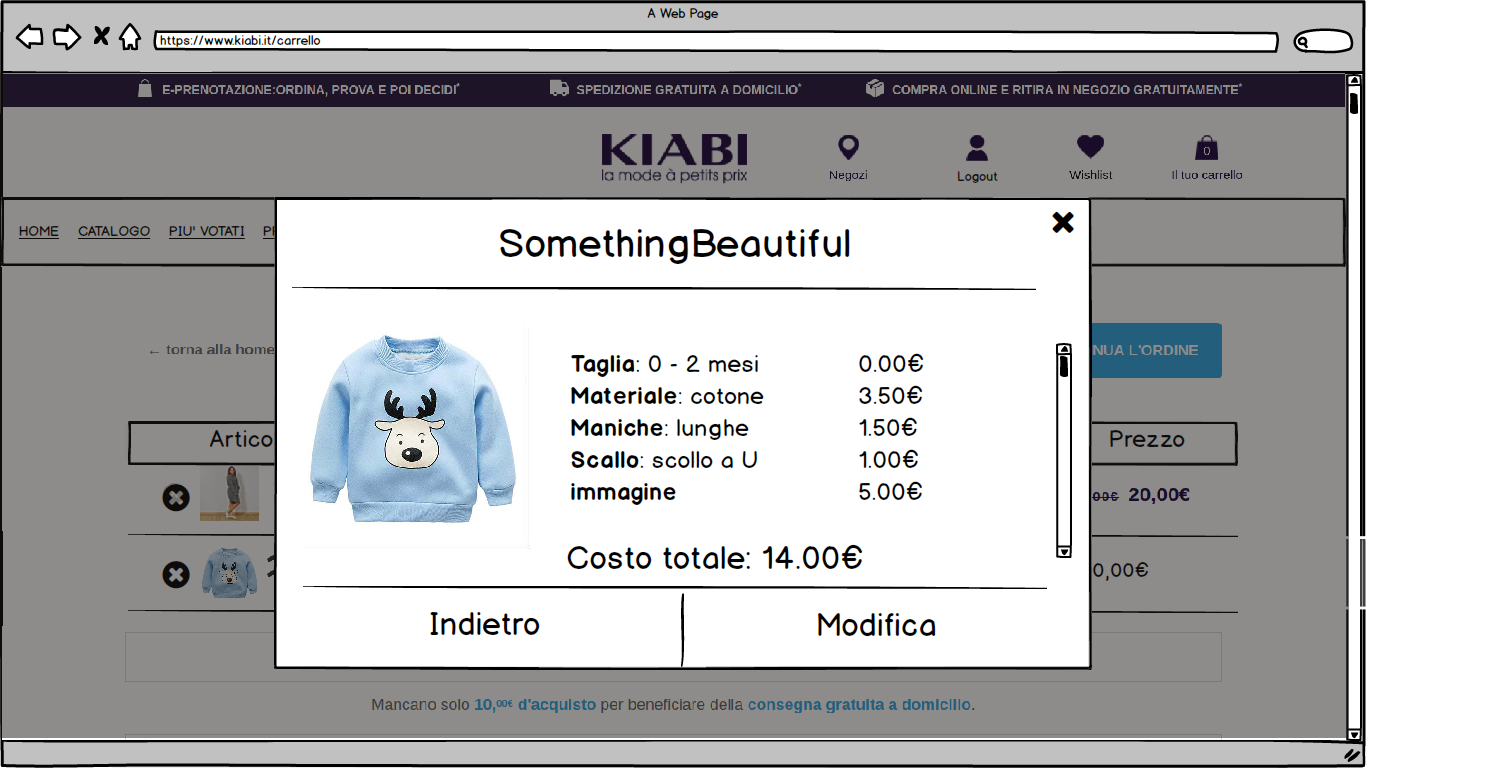
\includegraphics{balsamiq/Carrello dettagli.png}
\subsection{Registrazione} 
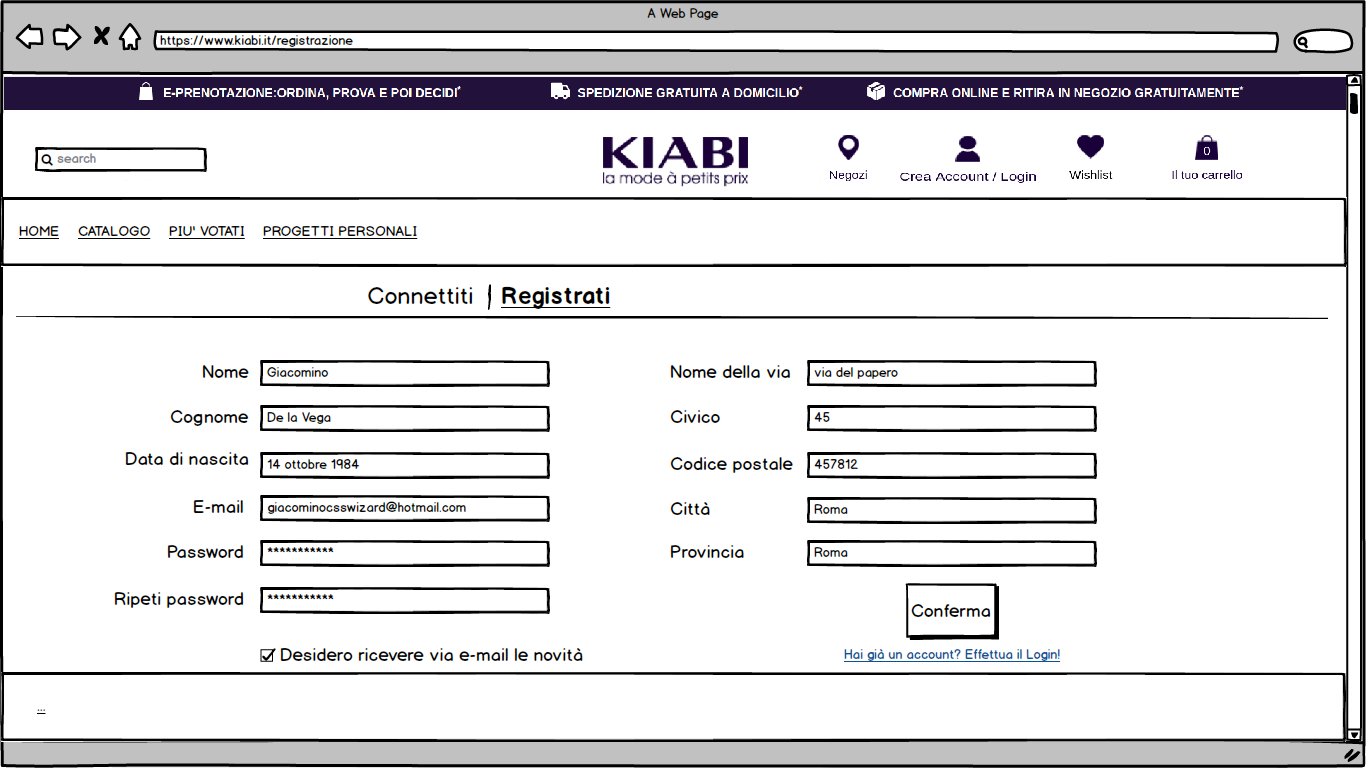
\includegraphics{balsamiq/Registrazione.png}
\end{document}
